\documentclass[a4paper,
11pt,  reqno]{amsart}
\usepackage[margin=1.2in,marginparwidth=1.5cm, marginparsep=0.5cm]{geometry}


\usepackage{amsmath,amssymb,amscd,amsthm,amsxtra, esint}
\usepackage{mathrsfs}
\usepackage[most]{tcolorbox}
\usepackage{color}
% \usepackage{showkeys}
\usepackage{hyperref}
\usepackage{subcaption}
% TO USE FIGURE FOR SOME TREES BUT WITH PLACEMENT SPECIFIER H SO THAT IT DOES NOT BEHAVE LIKE A FLOAT
\usepackage{float}

%\usepackage[notcite,notref]{showkeys}
\usepackage{bbm}
\usepackage{forest}
\newcommand{\red}{\color{red}}
\newcommand{\blue}{\color{blue}}
\newcommand{\fia}{\mathbbm{1}_{|\Phi-\alpha|<M}}
\newcommand{\psia}{\mathbbm{1}_{|\Psi-\alpha|<M}}
\newcommand{\jap}[1]{\langle #1 \rangle}
\newcommand{\I}{\hspace{0.2mm}\textup{I}\hspace{0.2mm}}
%Roman II
\newcommand{\II}{\textup{I \hspace{-2.9mm} I} }
%%Roman III
\newcommand{\III}{\textup{I \hspace{-2.9mm} I \hspace{-2.9mm} I}}
%
%%Roman IV
\newcommand{\IV}{\textup{I \hspace{-2.9mm} V}}
%%Roman V
\newcommand{\5}{\textup{V}}

\newcommand{\VI}{\text{V\hspace{-1.6mm} I}}

\newcommand{\noi}{\noindent}
\newcommand{\m}[1]{
	\ifdefequal{#1}{1}
	{\mathbbm{#1}}
	{\mathbb{#1}}
}
\newcommand{\FL}{\mathcal{F} L}
\newcommand{\ft}{\widehat}
\newcommand{\ind}{\mathbbm 1}
\newcommand{\les}{\lesssim}
\newcommand{\dl}{\delta}
\newcommand{\F}{\mathcal{F}}
\newcommand{\eps}{\varepsilon}
\DeclareMathOperator*{\intt}{\int}
\newcommand{\wt}{\widetilde}
\newcommand{\embeds}{\hookrightarrow}
\newcommand{\dx}{\partial_x}
\newcommand{\dt}{\partial_t}
\newcommand{\jp}{\color{orange}}

\allowdisplaybreaks[2]

%%%% FROM COW22
\newtheorem{theorem}{Theorem} [section]
\newtheorem{maintheorem}{Theorem}
\newtheorem{lemma}[theorem]{Lemma}
\newtheorem{proposition}[theorem]{Proposition}
\newtheorem{example}{Example}
\newtheorem{exercise}{Exercise}
\newtheorem{definition}[theorem]{Definition}
\newtheorem{corollary}[theorem]{Corollary}
\newtheorem{notation}{Notation}[section]
\newtheorem{claim}[theorem]{Claim}


\newtheorem{problem}{Problem}

\newtheorem{conjecture}{Conjecture}[section]
\newtheorem{scheme}{Scheme}[section]

\theoremstyle{remark}
\newtheorem{remark}[theorem]{Remark}




%Lower/Upper bound appears below /above the integral sign
\DeclareMathOperator*{\supp}{supp}
\DeclareMathOperator{\med}{med}
\DeclareMathOperator*{\ess}{ess}
\DeclareMathOperator*{\Area}{Area}
\DeclareMathOperator{\MAX}{MAX}


\DeclareMathOperator{\Id}{\rm Id}
\DeclareMathOperator{\sgn}{sgn}

\usepackage{mathtools}
\mathtoolsset{showonlyrefs=true}

\newcommand{\Z}{\mathbb{Z}}
\newcommand{\R}{\mathbb{R}}
\newcommand{\CC}{\mathbb{C}}
\newcommand{\T}{\mathbb{T}}
\newcommand{\bul}{\bullet}



\let\Re=\undefined\DeclareMathOperator*{\Re}{Re}
\let\Im=\undefined\DeclareMathOperator*{\Im}{Im}

\DeclareMathOperator{\com}{\textsf{com}}


\let\P= \undefined
\newcommand{\P}{\mathbf{P}}

\newcommand{\E}{\mathbb{E}}


\renewcommand{\L}{\mathcal{L}}



\newcommand{\LA}{\Lambda}

\newcommand{\aA}{\mathbf{A}^{\hspace{-0.75mm} 1}}

\newcommand{\bA}{\mathbf{A}^{\hspace{-0.75mm} 2}}


\newcommand{\bfA}{\mathbf{A}}

\newcommand{\K}{\mathcal{K}}
\newcommand{\TT}{\mathcal{T}}
\newcommand{\Tr}{\mathrm{T}}



\newcommand{\Nf}{\mathfrak{N}}
\newcommand{\fn}{\mathfrak{n}}

\newcommand{\Rf}{\mathfrak{R}}
\newcommand{\Hf}{\mathfrak{H}}


\newcommand{\hf}{\mathfrak{h}}
\newcommand{\hei}{\textup{height}}


\def\norm#1{\|#1\|}

\newcommand{\al}{\alpha}
\newcommand{\be}{\beta}

\newcommand{\nb}{\nabla}


\newcommand{\scrC}{\mathscr{C}}
\newcommand{\scrD}{\mathscr{D}}

\newcommand{\scrH}{\mathscr{H}}


\newcommand{\Dl}{\Delta}

\newcommand{\kk}{\kappa}
\newcommand{\g}{\gamma}
\newcommand{\G}{\Gamma}
\newcommand{\bG}{\mathbf{\Gamma}}
\newcommand{\ld}{\lambda}
\newcommand{\Ld}{\Lambda}
\newcommand{\s}{\sigma}

\newcommand{\zb}{\mathbf{z}}

\newcommand{\yb}{\mathbf{y}}


\newcommand{\ub}{\mathbf{u}}



\newcommand{\Xa}{\mathbf{X}}

\newcommand{\Xab}{\mathbf{X}^{\hspace{-0.4mm}\mathfrak{b}}}
\newcommand{\Xaa}{\mathbf{X}^{\hspace{-0.4mm}\mathfrak{g}}}

%%%% START OF NEW MACROS 
\newcommand{\bfrak}{\mathfrak{b}}
\newcommand{\gfrak}{\mathfrak{g}}
\newcommand{\Sf}{\mathfrak{S}}
\newcommand{\OPP}{\mathcal{B}}
\newcommand{\LOP}{\mathcal{L}}


\newcommand{\Xabe}{\mathbf{X}^{\hspace{-0.4mm}(\varepsilon),\mathfrak{b}}}
\newcommand{\Xaae}{\mathbf{X}^{\hspace{-0.4mm}(\varepsilon),\mathfrak{g}}}


\newcommand{\vb}{\mathbf{v}}
\newcommand{\wb}{\mathbf{w}}

\newcommand{\pb}{\mathbf{p}}
\newcommand{\gb}{\mathbf{g}}
\newcommand{\sbf}{\mathbf{s}}

%%%% END OF NEW MACROS ADDED 


\newcommand{\bbX}{\mathbb{X}}
\newcommand{\bbL}{\mathbb{L}}


\newcommand{\bbXa}{\mathbb{X}^{\hspace{-0.4mm}\mathfrak{g}}}
\newcommand{\bbXb}{\mathbb{X}^{\hspace{-0.4mm}\mathfrak{b}}}


\newcommand{\bbW}{\mathbb{W}}


\newcommand{\Xb}{\mathbf{X}^{\hspace{-0.4mm}2}}

\newcommand{\Xbc}{\mathbf{X}^3}


\newcommand{\Ta}{\mathbf{T}}

\newcommand{\Taa}{\mathbf{T}^{\mathfrak{g}}}

\newcommand{\Tab}{\mathbf{T}^{\mathfrak{b}}}


\newcommand{\Tb}{\mathbf{T}^2}
\newcommand{\Tba}{\mathbf{T}^{2,\mathfrak{g}}}
\newcommand{\Tbb}{\mathbf{T}^{2,\mathfrak{b}}}



\newcommand{\Tc}{\mathbf{T}^3}


\newcommand{\bv}{\big|}


\newcommand{\Bv}{\Big|}


\newcommand{\Si}{\Sigma}

\newcommand{\wh}{\widehat}

\newcommand{\Ft}{{\mathcal{F}}}

\newcommand{\cj}{\overline}

\newcommand{\dd}{\partial}
\newcommand{\invft}[1]{\overset{\vee}{#1}}
\newcommand{\lrarrow}{\leftrightarrow}

\newcommand{\LRA}{\Longrightarrow}
\newcommand{\LLA}{\Longleftarrow}
\newcommand{\LLRA}{\Longleftrightarrow}


\newcommand{\hC}{\widehat{\mathcal{C}}}


\newcommand{\ud}{\underline}

\newcommand{\btl}{\blacktriangleleft}



\newcommand{\ta}{\theta}

\renewcommand{\l}{\ell}
\renewcommand{\o}{\omega}


\newcommand{\Om}{\Omega}



\newcommand{\ges}{\gtrsim}


\newcommand{\wto}{\rightharpoonup}

%Japanese Bracket
\newcommand{\jb}[1]
{\langle #1 \rangle}




%
%bracket 2
\newcommand{\jbb}[1]
{[\hspace{-0.6mm}[ #1 ]\hspace{-0.6mm}]}



\renewcommand{\b}{\beta}


\renewcommand{\S}{\mathcal{S}}



\newcommand{\gf}{\mathfrak{g}}

\newcommand{\fc}{\mathfrak{c}}
\newcommand{\af}{\mathfrak{a}}

\newcommand{\fb}{\mathfrak{b}}


\newcommand{\ff}{\mathfrak{f}}




\newcommand{\pa}{\partial}
\newcommand{\pP}{\mathbf{P}}
\newcommand{\M}{\mathcal{M}}
\newcommand{\MMb}{\mathbf{M}}
\def\e{\eps}

\newcommand{\N}{\mathbb{N}}

\newcommand{\oet}{(\omega|_{M})_{\eta}}
\newcommand{\oget}{(\omega|_{M})_{g\cdot\eta}}
\newcommand{\ze}{\zeta}


\newcommand{\Pk}{P^{(2m)}_2}
\newcommand{\Pkn}{P^{(2m)}_{2, N}}
\newcommand{\Hcal}{\mathcal{H}}
\newcommand{\Li}{L^{(1)}}

\DeclareMathOperator{\Lip}{Lip}





\DeclareMathOperator{\mul}{mul}
\DeclareMathOperator{\mulB}{mul_{\BB}}



% OTHER OPTION FOR TREES

\tikzset{
	dotA/.style={
		transform shape, fill,circle,inner sep=1.5pt, label distance=-1pt,
		%	transform shape,inner sep=0pt, label distance=-1pt,
		font={\normalsize }
	},
	>=stealth,
}

\tikzset{
	dotAB/.style={
		transform shape, fill,circle,inner sep=1.5pt, label distance=-10pt,
		%	transform shape,inner sep=0pt, label distance=-1pt,
		font={\small }
	},
	>=stealth,
}

\makeatletter
\def\DeclareSymbolNew#1#2#3#4#5{\expandafter\gdef\csname MH@symb@#1\endcsname{\tikz[baseline=#2,scale=0.5, every node/.style={dotA},
		level distance=15pt,
		level 1/.style={sibling distance=#3pt},
		level 2/.style={sibling distance=#4pt},
		level 3/.style={sibling distance=15pt}
		]{#5}}}
\def\<#1>{\csname MH@symb@#1\endcsname}
\makeatother


% Variables that determine the distance between the each generation of nodes
\def\distC{15}




\DeclareSymbolNew{1}{-7}{\distC}{\distC}
{
	\node   (root) {}
	child
	child
	;
	\node  at (root-1) {};
	\node at (root-2) {};
}

\DeclareSymbolNew{11}{-7}{\distC}{\distC}
{
	\node   (root) {}
	child
	child
	;
	\node  at (root-1) {};
	\node at (root-2) {};
}

\newcommand{\cherryS}{
	\resizebox{!}{1.3ex}{%
		\<1>%
	}
}

\newcommand{\starT}{
	
\begin{tikzpicture}[
		baseline=-3, scale=1, every node/.style={dotAB},
		]
		\node  [label={}, transform shape, star,transform shape, star, star point ratio=2.25,inner sep=1pt, label distance=-1pt]  (root) {};
	\end{tikzpicture}
}


%cherry with labels
\newcommand{\cherry}[3]{
	\begin{tikzpicture}[
		baseline=-8, scale=0.6, every node/.style={dotA},
		level distance=15pt,
		level 1/.style={sibling distance=\distC pt}
		]
		\node  [label=above:{$#1$}]  (root) {}
		child
		child
		;
		\node [label= left:{$#2$}]  at (root-1) {};
		\node [label= right:{$#3$}] at (root-2) {};
	\end{tikzpicture}
}


\DeclareSymbolNew{01}{-7}{\distC}{\distC}
{
	\node  [circle,draw=black, fill=white, inner sep=0pt,minimum size=7pt]  (root) {}
	child  child;
	\node  at (root-1) {};
	\node at (root-2) {};
}

\DeclareSymbolNew{21}{-12}{\distC}{\distC}
{
	\node   (root) {}
	child {child child} child;
	\node  at (root-1) {};
	\node at (root-2) {};
	\node  at (root-1-1) {};
	\node at (root-1-2) {};
}

\DeclareSymbolNew{22}{-12}{\distC}{\distC}
{
	\node   (root) {}
	child child {child child};
	\node  at (root-1) {};
	\node at (root-2) {};
	\node  at (root-2-1) {};
	\node at (root-2-2) {};
}

\DeclareSymbolNew{31}{-12}{\distC}{\distC}
{
	\node   (root) {}
	child {child {child child} child} child;
	\node  at (root-1) {}; \node at (root-2) {};
	\node at (root-1-1) {}; \node at (root-1-2) {};
	\node  at (root-1-1-1) {}; \node at (root-1-1-2) {};
}

\DeclareSymbolNew{32}{-12}{\distC}{\distC}
{
	\node   (root) {}
	child {child child {child child} } child;
	\node  at (root-1) {}; \node at (root-2) {};
	\node at (root-1-1) {}; \node at (root-1-2) {};
	\node  at (root-1-2-1) {}; \node at (root-1-2-2) {};
}

\DeclareSymbolNew{33}{-12}{21}{\distC}
{
	\node   (root) {}
	child {child child} child {child child};
	\node  at (root-1) {}; \node at (root-2) {};
	\node at (root-1-1) {}; \node at (root-1-2) {};
	\node  at (root-2-1) {}; \node at (root-2-2) {};
}

\DeclareSymbolNew{34}{-12}{\distC}{\distC}
{
	\node   (root) {}
	child child {child {child child} child  } ;
	\node  at (root-1) {}; \node at (root-2) {};
	\node at (root-2-1) {}; \node at (root-2-2) {};
	\node  at (root-2-1-1) {}; \node at (root-2-1-2) {};
}

\DeclareSymbolNew{35}{-12}{\distC}{\distC}
{
	\node   (root) {}
	child child {child child {child child} } ;
	\node  at (root-1) {}; \node at (root-2) {};
	\node at (root-2-1) {}; \node at (root-2-2) {};
	\node  at (root-2-2-1) {}; \node at (root-2-2-2) {};
}






%--------------------------------------------------------------------

\newtheorem*{ackno}{Acknowledgements}











\newcommand{\J}{\mathcal{J}}
\newcommand{\If}{\mathfrak{I}}
\newcommand{\Jf}{\mathfrak{J}}
\newcommand{\Af}{\textgoth{A}}
\newcommand{\RR}{\mathcal{R}}
\newcommand{\B}{\mathcal{B}}
\newcommand{\Ical}{\mathcal{I}}



\newcommand{\NR}{\textit{NR}}


\newcommand{\A}{\mathcal{A}}

\newcommand{\Gc}{\mathcal{G}}

\newcommand{\C}{\mathcal{C}}
\numberwithin{equation}{section}
\numberwithin{theorem}{section}


%%%

\newcommand{\Q}{\mathbb{Q}}
\newcommand{\PP}{\mathbb{P}}


\DeclareMathOperator{\Law}{Law}

\newcommand{\ZZ}{\mathfrak{Z}}
\newcommand{\WW}{\mathfrak{W}}


\newcommand{\muu}{\vec{\mu}}
\newcommand{\muuu}{\vec{\wt{\mu}}}

\newcommand{\rhoo}{\vec{\rho}}
\newcommand{\rhooo}{\overrightarrow{{\rho}^\dia}}
\newcommand{\rhoooN}{\overrightarrow{{\rho}_N^\dia}}



\newcommand{\hra}{\hookrightarrow}

\newcommand{\V}{\mathcal{V}}
\newcommand{\W}{\mathcal{W}}
\newcommand{\U}{\mathcal{U}}

\newcommand{\dr}{\theta}
\newcommand{\Dr}{\Theta}

\newcommand{\Ha}{\mathbb{H}_a}
\newcommand{\Hc}{\mathbb{H}_c}

\newcommand{\MM}{\mathrm{M}}
\newcommand{\NN}{\mathrm{N}}
\newcommand{\Ncal}{\mathcal{N}}
\newcommand{\BB}{\mathrm{B}}
\newcommand{\D}{\mathrm{D}}
\newcommand{\DD}{\mathcal{D}}

\newcommand{\Res}{\mathfrak{R}}
\newcommand{\Qxy}{Q_{X,Y}}
\newcommand{\qxy}{q_{X,Y}}

\newcommand{\QN}[1]{Q_{N_#1}}
\newcommand{\QxyN}{Q_{X_N,Y_N}}
\newcommand{\Qk}[1]{Q_{X_{N_{#1}},Y_{N_{#1}}}}


\newcommand{\Qu}{\wt Q}


\newcommand{\wIf}{\wt \If_{\pl, \pe}}
\newcommand{\wIfN}{\wt \If_{\pl, \pe, N}}
\newcommand{\Kf}{\mathfrak K}


\newcommand{\dia}{\diamond}
\newcommand{\Y}{\bY}

\newcommand{\Bf}{\mathfrak B}

\newcommand{\bW}{\mathbb W}

\newcommand{\bfW}{\mathbf W}



\newcommand{\LHS}{\mathcal{L}_{\rm HS}}





\newcommand{\bX}{\mathbb X}

\newcommand{\bY}{\mathbb Y}

\newcommand{\cP}{\mathcal P}

\newcommand{\cQ}{\mathcal Q}


\newcommand{\cZ}{\mathcal Z}

\newcommand{\too}{\longrightarrow}

\newcommand{\proj}{\Pi}

\newcommand{\Ups}{\Upsilon}
\newcommand{\UUps}{{\ud \Upsilon}}

\newcommand{\Ab}{\mathbb{A}}
\newcommand{\Psii}{\Psi \hspace{-2.55mm}\Uppsi}

\newcommand{\RN}{\mathfrak{R}}
\newcommand{\ldd}{\vec \ld}

\newcommand{\plan}{\mathfrak{p}}

\newcommand{\Xc}{\mathcal{X}}

\newcommand{\Zc}{\cZ}
\newcommand{\ba}{\pmb{a}}
\newcommand{\hJ}{\mathcal{J}}



\newcommand{\pPsi}{\mathbf{\Psi}}


\newcommand{\XX}{\mathbf{X}}
\newcommand{\YY}{\mathbf{Y}}

\newcommand{\uu}{\pmb{u}}
\newcommand{\w}{{\rm w}}


\newcommand{\WP}{W^\Phi}


\newcommand{\ssq}{\scaleto{\square}{3.5pt}}



\newcommand{\andreia}[1]{\marginpar{\color{purple} $\Leftarrow\Leftarrow\Leftarrow$}{\smallskip \noi\color{purple}ANDREIA: #1}\smallskip}
\newcommand{\simao}[1]{\marginpar{\color{red} $\Leftarrow\Leftarrow\Leftarrow$}{\smallskip \noi\color{red}SIMAO: #1}\smallskip}
\newcommand{\joao}[1]{\marginpar{\color{brown} $\Leftarrow\Leftarrow\Leftarrow$}{\smallskip \noi\color{red}JOAO: #1}\smallskip}






\makeatletter
\@namedef{subjclassname@2020}{%
	\textup{2020} Mathematics Subject Classification}
\makeatother


\title{Sharp local well-posedness for the Novikov-Veselov equation}


\title[Sharp LWP for the Novikov-Veselov equation]{Sharp local well-posedness for the Novikov-Veselov equation}
\author[A.~Chapouto \and S.~Correia \and J.~P.~Ramos]
{Andreia Chapouto \and Sim\~ao Correia \and Jo\~ao Pedro Ramos}


\date{\today}


\address{Andreia Chapouto,
	CNRS, and Laboratoire de math\'ematiques de Versailles, UVSQ, Universit\'e Paris-Saclay, CNRS, 45 avenue des \'Etats-Unis, 78035 Versailles Cedex, France}

\email{andreia.chapouto@uvsq.fr}

\address{Sim\~ao Correia,
	Center for Mathematical Analysis, Geometry and Dynamical Systems,
	Department of Mathematics,
	Instituto Superior T\'ecnico, Universidade de Lisboa
	Av. Rovisco Pais, 1049-001 Lisboa, Portugal
}

\email{simao.f.correia@tecnico.ulisboa.pt}

\address{Jo\~ao Pedro Ramos, 
	IMPA, Rio de Janeiro, Brazil}

\email{joao.ramos@impa.br}




\subjclass[2020]{35A01, 35A22, 35Q53, 37K10}



\keywords{Novikov-Veselov equation, gauge transform,
	local well-posedness.
}
\begin{document}
\maketitle
\begin{abstract}
	We prove that the (nonzero) Novikov-Veselov equation is locally well-posed for initial data $u_0\in H^s(\R^2)$ in the full subcritical range $s>-1$, by introducing a suitable gauge transform. The resulting gauged equation, despite having infinitely many nonlinear terms, is shown to be controllable at low regularity in the usual Fourier restriction norm framework. In particular, the result is perturbative and does not rely on the complete integrability structure of the Novikov-Veselov equation.
\end{abstract}

\section{Introduction}
\subsection{Setting of the problem and main results}
We consider the Novikov-Veselov equation on $\R^2$,
\begin{equation}\tag{NV}\label{eq:NV}
	\partial_t u + (\partial^3 + \overline{\partial}^3)u + \frac34(\partial(u\overline{\partial}^{-1}\partial u) + \overline{\partial}(u\partial^{-1}\overline{\partial}u)) + E(\overline{\partial}^{-1}\partial^2 u + \partial^{-1}\overline{\partial}^2 u)=0,
\end{equation}
with initial data $u_0\in H^s(\R^2)$, where $\partial=\frac12(\partial_x+i\partial_y)$,
$\overline{\partial}=\frac12(\dx-i\partial_y)$, and $E\in \R$ is the
\emph{energy} parameter.

\medskip

The Novikov-Veselov equation was introduced, in implicit form, by Novikov and Veselov \cite{NovikovVeselov} (see also Manakov
\cite{Manakov}) as a
$(2+1)$-dimensional completely integrable analogue of the Korteweg-de Vries equation, associated with the
two-dimensional inverse scattering problem for the Schr\"odinger operator. In particular,
if $u$ is independent of the $y$-variable, then \eqref{eq:NV} reduces to the classical KdV
equation on the line. This places \eqref{eq:NV} among the standard higher-dimensional
dispersive generalizations of KdV, together with the Kadomtsev-Petviashvilii and
Zakharov-Kuznetsov equations; see, for instance,
\cite{bourg_kpii, takaokaTzvetkov, HHK, IonescuKenigTataru, GuoPengWang,
Kinoshita_ZK}. At the same time, the nonlocal structure of \eqref{eq:NV} and the geometry
of its two-dimensional resonances give it a distinct analytic profile, even when compared
with other quadratic models.

\medskip



There are two natural ways to view \eqref{eq:NV}. One is integrable: inverse scattering,
Miura-type transforms and the modified Novikov-Veselov hierarchy provide access to
existence and long-time questions. The other is perturbative: one treats \eqref{eq:NV} as
a semilinear dispersive equation and asks how far robust Fourier-analytic methods can be
pushed without using complete integrability. The main purpose of this paper is to show
that, for the local Cauchy problem, the perturbative point of view is strong enough to
recover the full subcritical Sobolev theory.

\medskip



Equation \eqref{eq:NV} is also connected to the physically relevant KP models. After a
suitable anisotropic rescaling, the formal high-energy limit $E\to +\infty$ leads to KP-I,
while $E\to -\infty$ leads to KP-II; see the discussion in
\cite{kazeykinamunoz1, kazeykinamunoz2}. This relation explains part of the interest in
the nonzero-energy equation, but from the low-regularity viewpoint the decisive feature is
still the scaling. Indeed, if $u$ solves \eqref{eq:NV} with energy $E$, then
\begin{equation}\label{scaling}
u_\lambda(t,x)=\lambda^2u(\lambda^3t,\lambda x),\quad \lambda>0,
\end{equation}
is again a solution, now with energy $\lambda^2E$. Hence, when $E=0$, the equation is
exactly scaling-invariant, and a direct computation shows that the homogeneous
$\dot H^s(\R^2)$ norm is preserved when $s=s_c=-1$. This makes $H^{-1}(\R^2)$ the
critical Sobolev scale for the zero-energy problem, and strongly suggests that local
well-posedness should hold throughout the subcritical range $s>-1$. For fixed nonzero
energy the scaling is not a symmetry, but the same exponent $s_c=-1$ still governs the
expected threshold.

\medskip



We now describe the existing literature. On the integrable side, the construction of
solutions through inverse scattering and related techniques goes back to
\cite{BLMP, Tsai, Perry, MusicPerry}.  In the zero-energy case, one may exploit the Miura map
\cite{Bogdanov},
\begin{equation}
\mathbf{M}[u]= 2\partial u + |u|^2,
\end{equation}
which maps solutions of the \emph{modified} Novikov-Veselov equation
\begin{equation}
\partial_t u + (\partial^3+\overline{\partial}^3) u + \frac34\left(\partial(u\overline{\partial}^{-1}\partial |u|^2) + \overline{\partial}(u\partial^{-1}\overline{\partial}|u|^2) + u\partial^{-1}\overline{\partial}(\overline{u}\overline{\partial}u) + u\overline{\partial}^{-1}\partial(\overline{u}\partial u)\right)=0\label{eq:mNV}\tag{mNV}
\end{equation}
satisfying $\partial u=\overline{\partial} u$ to solutions of \eqref{eq:NV} with $E=0$. 
Since \eqref{eq:mNV} is cubic, its local theory is much better behaved at low regularity:
Schöttdorf \cite{Schottdorf} proved small data global well-posedness for \eqref{eq:mNV} in the critical space $L^2(\R^2)$;
see also \cite{MPS_Dysthe, CorreiaKinoshita} for analogous critical results in other
2d cubic dispersive models. More recently, Nachman, Perry and Tataru
\cite{NPT_mNV} extended Schöttdorf's result to large-data global well-posedness for the modified
Novikov-Veselov system. By the Miura map, this leads to existence
results for the zero-energy \eqref{eq:NV} for a particular class of large initial data in $H^{-1}(\R^2)+L^1(\R^2)$.

\medskip



This transfer of well-posedness from a modified equation to the original one is analogous to the Miura-map
theory for KdV \cite{Miura, KPST_miura, CKSTT_sharp_kdv, KT06, BuckmasterKoch,
KillipVisan_kdv}. There is, however, a substantial difference between the two problems.
For KdV, complete integrability comes with coercive conservation laws, and this ultimately
permits a global theory down to $H^{-1}(\R)$, which is optimal by \cite{Molinet_ill_line}.
For \eqref{eq:NV}, on the contrary, the conserved quantities are not coercive, and this is
consistent with the existence of blow-up solutions \cite{TaimanovTsarev}. Thus, while the
integrable structure is extremely informative, it does not settle the semilinear
low-regularity Cauchy problem for \eqref{eq:NV}.

\medskip



If one restricts attention to contraction or fixed-point arguments, the picture before this
work was substantially weaker. For nonzero energy, Kazeykina and Mu\~noz proved in
\cite{kazeykinamunoz1, kazeykinamunoz2} local well-posedness for $s>\frac12$, using
refined stationary-phase estimates adapted to the geometry of the dispersive symbol. Independently,
Angelopoulos \cite{angelopolous} reached the endpoint $s=\frac12$ in Bourgain-type
spaces. In the zero-energy case, Adams and Gr\"unrock \cite{adamsgrunrock} exploited the
simpler resonance relation to prove local well-posedness for $s>-\frac34$. All these
results remain far above the scaling threshold $s=-1$. On the negative side,
Angelopoulos also proved in \cite{angelopolous} that for $s<-1$ the data-to-solution map
cannot be analytic at the origin, ruling out fixed-point constructions below scaling.
Hence the subcritical gap prior to this work is
\[
-1< s\le \frac12 \quad \text{for } E\neq 0,
\qquad
-1< s\le -\frac34 \quad \text{for } E=0.
\]

\medskip



The main result of this paper closes this gap completely.


\begin{theorem}\label{thm:main_intro}
    Fix $E\in\R$ and $s>-1$. Given $u_0\in H^s(\R^2)$, there exists $T=T(\|u_0\|_{H^s})$ and $u\in C([0,T]; H^s(\R^2))$ such that, for any sequence $u_{0,n}\in \mathcal{S}(\R^2)$, with $u_{0,n}\to u_0$ in $H^s$, the corresponding solutions $u_n$ to \eqref{eq:NV} (given by \cite{angelopolous, kazeykinamunoz1, kazeykinamunoz2}) are defined on $[0,T]$ and $u_n\to u$ in the $C_tH^s$ topology. Moreover, the resulting \eqref{eq:NV} flow $u_0\in H^s\mapsto u\in C_tH^s$ is analytic.
\end{theorem}


\begin{remark}
We stress that Theorem \ref{thm:main_intro} is of \emph{semilinear} nature and is
completely independent of the complete integrability structure of \eqref{eq:NV}.
\end{remark}


\begin{remark}
The endpoint $s=-1$ remains open. Critical well-posedness is known for several other
cubic two-dimensional dispersive equations, for instance for \eqref{eq:mNV}
\cite{Schottdorf}, for KP-II \cite{HHK}, for the Dysthe equation \cite{MPS_Dysthe}, and
for the modified Zakharov-Kuznetsov equation \cite{CorreiaKinoshita}, using the $U^2-V^2$ framework of Koch-Tataru \cite{KochTataru} (but is yet to be achieved for quadratic cases). In our setting, the main difficulty arises in controlling nonlinear terms of any order greater than two, each of them presenting critical decay in frequency, leading to arbitrarily many logarithmic divergences.
\end{remark}


\subsection{Overview of the method}


The proof of Theorem \ref{thm:main_intro} builds upon the strategy developed in our recent
work on KdV \cite{chcora} (which improved the well-posedness theory in Fourier-Lebesgue spaces $\FL^{s,p}(\R)$, $p>2$), but the present problem contains a genuinely new phenomenon:
for Novikov-Veselov, the same mechanism improves the Sobolev theory all the way down to
the scaling threshold. The argument combines infinite normal form reductions, a gauge
transform, and multilinear estimates of Fourier-restriction type. The normal-form
component is in the spirit of Babin--Ilyin--Titi \cite{bit} and of the later developments
\cite{GKO13, KOY20, OW21, Kishimoto22}, while the analytic estimates are adapted to the
frequency-restricted framework of \cite{COS}.


Passing to the interaction representation, we define
\[
v(t):=\F_z\big(U(-t)u(t)\big),
\]
where $U(t)$ denotes the linear propagator associated with \eqref{eq:NV}. The quadratic
nonlinearity is then governed by the phase
\[
\Phi(\xi,\xi_1,\xi_2)=\Phi_0(\xi,\xi_1,\xi_2)+E\Phi_E(\xi,\xi_1,\xi_2),\quad \xi, \xi_1, \xi_2\in \R^2\simeq \CC,
\]
with
\[
\Phi_0(\xi,\xi_1,\xi_2)=\Re(-\xi^3+\xi_1^3+\xi_2^3)=-3\Re(\xi\xi_1\xi_2),
\]
and
\[
\Phi_E(\xi,\xi_1,\xi_2)
=-\Re\Big(-\frac{\xi^3}{|\xi|^2}+\frac{\xi_1^3}{|\xi_1|^2}+\frac{\xi_2^3}{|\xi_2|^2}\Big).
\]
The corresponding bilinear multiplier is
\[
K(\xi_1,\xi_2)=\frac{\xi_1\cdot\xi_2}{|\xi_1|^2|\xi_2|^2}.
\]
Thus \eqref{eq:NV} becomes, schematically,
\begin{equation}\label{eq:NV2}
	v(t,\xi)=v(0,\xi)+\int_0^t \int_{\xi=\xi_1+\xi_2} e^{it'\Phi}K\Phi_0\,v(t',\xi_1)v(t',\xi_2)\,d\xi_1dt'.
\end{equation}


The key algebraic observation is the identity
\[
K\Phi_0=K\Phi-EK\Phi_E.
\]
The term containing $K\Phi_E$ is perturbative, since $\Phi_E$ is effectively of lower
order than $\Phi_0$. The difficult contribution is the one containing $K\Phi$ and is responsible for the obstructions in the aforementioned literature. However, it
invites a differentiation by parts in time through
\[
e^{it\Phi}=\frac{\partial_t e^{it\Phi}}{i\Phi}.
\]
If one performed this step naively on the whole frequency space, one would create
artificial singularities near the resonance set $\{\Phi=0\}$. To avoid this, we split the
convolution region into a good set, where the multiplier itself has sufficient structure to be estimated directly, and a bad set, where division by $\Phi$ is harmless.


Iterating this procedure generates an infinite normal form expansion indexed by binary
trees. Each iteration gains one power of the phase in the denominator, but at the price of
producing boundary terms. These boundary contributions are the main obstacle to closing a
contraction argument at $s>-1$. The central idea of the paper is that they can be removed
through a nonlinear change of variables, namely a gauge transform $\Gc_\delta$ built from
the full normal form series. For smooth small solutions, the original variable and the
gauged variable remain equivalent, but the transformed equation has a much better
structure at low regularity: the worst quadratic interactions are cancelled and replaced by
a hierarchy of multilinear terms whose symbols are compatible with frequency-restricted
estimates.


Once the gauged equation is derived, its local theory is obtained by a fixed-point
argument in short-time $X^{s,b}$-type spaces. The multilinear analysis uses a detailed
study of the NV resonance geometry together with a systematic organization of tree
contributions according to their algebraic type. This yields a locally analytic flow for the
gauged equation below all previously known thresholds. Finally, one inverts the gauge map
in the same range $s>-1$ and transfers the result back to the original Novikov-Veselov
equation. In this way, one obtains a sharp subcritical local well-posedness theory for
\eqref{eq:NV} by purely perturbative means, with no appeal to inverse scattering or to the
complete integrability machinery.




\bigskip


\subsection{Acknowledgements} 
The authors are deeply indebted to Axel Grünrock for his encouragement and for several important discussions.

\medskip

A.~C. was partially supported by  CNRS-INSMI through a grant ``PEPS Jeunes chercheurs et jeunes chercheuses 2025". S.~C. was partially supported by Funda\c{c}\~ao para a Ci\^encia e Tecnologia (FCT), through CAMGSD (project UID/04459/2025). A. C. and S. C. were also supported by FCT, through the grant FCT/Mobility/1330917020 /2024-25). A.~C. is thankful for the kind hospitality of Instituto Superior Técnico, where part of this work was developed. S.~C. and J.~P.~R. were also supported by FCT through project SHADE (project 2023.17881.ICDT, DOI  10.54499/2023.17881.ICDT).










\section{Preliminaries}\label{sec:prem}


\subsection{Tree formalism}	
\label{SUB:tree}





\begin{definition}
\label{DEF:tree}
\rm 
A \emph{binary tree} $\TT$ is a partially ordered set (with partial order $\le$) satisfying the following properties:

\begin{enumerate}
\item[(i)] $\TT$ has a unique minimal element called the \textit{root node} labelled by $\emptyset$ (i.e., $\emptyset \le a$ for all $a \in \TT$). 

\smallskip 
\item[(ii)] Given $a\in \TT\setminus \{ \emptyset \}$, 
there exists a unique $b \in \TT$ such that: $b\ne a$, $b \le a$, and $b \le c \le a$ implies $c\in\{a,b\}$. In that case, we say that $b$ is the \textit{parent} of $a$ and $a$ is a \textit{child} of $b$. 

\smallskip 
\item[(iii)] A node $a\in \TT$ is called \textit{terminal} or a \textit{leaf} if it has no children. A \textit{non-terminal node} or a \textit{parent} $a\in\TT$ is a node with exactly two children, one called \textit{left child} and the other \textit{right child}.\footnote{Introducing the notation of left and right children of a node  reflects the lack of ambiguity in the usual planar representation of binary trees.}  
We write $\TT^0, \TT^\infty$ for the sets of parent and terminal nodes of $\TT$, respectively.  Note that $\TT$ is the disjoint union of $\TT^0$ and $\TT^\infty$. 

\smallskip 
\item[(iv)]
Each node in $\TT$ is labelled with a word in the following way: the root node has word~$\emptyset$; and for a given parent node $a\in \TT^0$, its left and right children have labels $a1$ and $a2$,  obtained by concatenating $1$ or $2$ to the right of $a$, respectively. Note that children of the root node have labels 1 and 2. 


\end{enumerate}



\noi
We interchangeably use $\TT$ to denote the representation of the tree as a finite connected graph and to denote the set of words used to label its nodes. Note that the latter is also a partially ordered set, with words $a,b$ satisfying $a\le b$ if there exists a word $c$ such that $b = ac$. 



\end{definition}


Given $j\in\N$, we use the notation $\Tr_j$ to denote the family of all binary trees
with $j$ non-terminal nodes, which we call the $j$-th generation of trees. From Definition~\ref{DEF:tree}, it follows that 
\begin{align}
| \TT^0 |  = j \quad \text{and} \quad |\TT^\infty| = j+1.
\end{align}


\noi
It is not difficult to see that the number of distinct trees in $\Tr_j$ is given by the $j$-th Catalan number
\begin{align}\label{eq:catalan}
| \Tr_j | = \frac{1}{j+1} \binom{2j}{j}  = \frac{(2j)!}{(j+1)! j !}.
\end{align}
In particular, the first 3 generations of trees are succintly written below, identified by their graphs:
\begin{align*}
\Tr_1 & = \big\{ \<1> \big\}, \\
\Tr_2 & = \left\{ \<21>, \<22> \right\}, \\
\Tr_3 &  = \left\{ \<31>, \<32>, \<33>, \<34>, \<35> \right\}.
\end{align*}
Similarly, we can represent the trees above by the following partially ordered sets of words used to label their nodes (as per Definition \ref{DEF:tree}(iv)):
\begin{align}
\<1> 
&
= \{\emptyset\}
, 
\\
\<21>
&
=
\{ \emptyset, 1 ,2, 11,12  \}
, 
\\
\<22>
&
=
\{\emptyset, 1,2, 21,22\}
, 
\\
\<31>
&
= 
\{
\emptyset, 1,2, 11,12, 111, 112
\}
, \ldots
\end{align}




\smallskip








For readibility, we will reserve the symbols $\bul$, $\star$, $\circ$, and $\ast$ to denote nodes in a tree and their respective associated word. 
Next, we introduce some additional notation to identify different nodes in a tree. 


\begin{definition}\rm
\label{DEF:tree2}
Let $\TT$ be a binary tree in the sense of Definition~\ref{DEF:tree} and 
$\bul, \star$ be two nodes in $\TT$. 

\begin{enumerate}



\smallskip
\item[(i)]
If $\bul \in \TT\setminus \{ \emptyset\}$, we write $\pb(\bul)$ to denote the \emph{parent node} of $\bul$. If $\pb(\star)\neq \emptyser$, we write $\gb(\bul)=\pb(\pb(\bul))$.

\smallskip
\item[(ii)] 
If $\bul, \star\in \TT \setminus\{ \emptyset \}$ are distinct and share the same parent, they are called \textit{siblings}. We write $\sbf(\bul)$ for the sibling of $\bul$. 

\smallskip
\item[(iii)] 
Given $\bul\in \TT^0$, we say $\bul$ is a \textit{final parent} if its children $\bul1, \bul2 \in \TT^\infty$. The set of final parents is denoted by $\TT^{0,\ff}$.


\end{enumerate}



\end{definition}


\begin{remark}\rm 
Note that from Definition~\ref{DEF:tree}, the maps $\pb, \sbf$, for the parent and sibling of a given node, are well-defined in their respective domains, since if either the parent or sibling node exists, it is unique. 

\end{remark}





We next introduce concatenation and subtraction of trees. 


\begin{definition} 
\label{DEF:tree3}
\rm

Let $\TT$ be a binary tree in the sense of Definition~\ref{DEF:tree}. 


\begin{enumerate}




\smallskip
\item[(i)] (Concatenation)  
Given $ \star \in \TT^\infty$, we define
$$
\TT \overset{\star}{\oplus} \<1>
: = \TT \cup \{\star1, \star2\}
$$
as the result of adding the children $\star1,\star2$ of $\star$ to the tree $\TT$. 
Note that this operation now makes $\star$ a final parent in the tree $\TT \overset{\star}{\oplus} \<1>$. 




\smallskip
\item[(ii)] (Subtraction) 
Given a final parent $\star  \in \TT^{0,\ff}$, we define the tree
$$
\TT \overset{\star }{\ominus } \<1>
: = \TT \setminus \{ \star1, \star2  \}
$$
as the result of eliminating the children $\star1, \star2$ of $\star$
from $\TT$. Note that $\star$ becomes a terminal node in the new tree $\TT \overset{\star}{\ominus } \<1>$. 
More generally, given $C\subseteq \TT^{0,f}$, we define
\begin{align}
\label{treeSubtr}
\TT \overset{C}{\ominus} \<1> : =
 \bigcap_{\star \in C} ( \TT \overset{\star}{\ominus}  \<1>)
= \bigcap_{\star\in C} (\TT \setminus \{\star1,\star2\})
= \TT \setminus \Big( \bigcup_{\star\in C} \{\star1,\star2\} \Big), 
\end{align}
which corresponds to the set where all the children of the final parents $\star\in C$ have been removed from the tree.


\end{enumerate}



\end{definition}



The tree structure defined above and its word-labelling will help in keeping track of the nonlinear terms appearing in our normal form reduction procedure. Namely, after an differentiation-by-parts step, a time derivative falls on a $v$-factor as in \eqref{NF00}, after which we use equation \eqref{dtv} to replace it by a quadratic term, generating a higher degree nonlinear contribution. We can then use binary trees to label the frequencies of the corresponding factors, in the following way. 


\begin{definition}\rm 

Let $j\in\N$ and $\TT \in \Tr_j$. 

\begin{enumerate}
\item[(i)] (Index function) 
We define the index function $\vec\xi : \TT\to \CC^\TT$ such that $\vec\xi = (\xi_\bul)_{\bul\in\TT}$, where
\begin{align}
\label{parent}
\xi_\bul = \xi_{\bul1} + \xi_{\bul2}, \quad \bul\in \TT^0,
\end{align}
and $\bul1$ and $\bul2$ denote the children of $\bul$. Moreover, we define the set $\G(\TT)$ as the set of convolution relations on the tree $\TT$:
\begin{align}
\label{Gamma}
\G(\TT) : = \big\{ \vec\xi \in \CC^\TT: \ \xi_\bul = \xi_{\bul1} + \xi_{\bul2}, \ \bul \in \TT^0 \big\}. 
\end{align}


\smallskip

\item[(ii)] (Zero-energy phase function) 
We use $\Psi(\TT)$ to denote the \textit{zero-energy phase function}associated with the tree $\TT$, given by
\begin{align}
\label{psi0-tree}
\Psi_0(\TT)
:=
\Re\left(- \xi^3 + \sum_{\bul\in \TT^\infty} \xi_\bul^3\right)
\end{align}
where $\TT^\infty$ denotes the set of leaves of $\TT$. 


Given a parent node $\star\in\TT^0$, we also introduce the partial zero-energy phase function for the tree $\cherry{\star}{}{}=\{\star, \star1, \star2\}$:
\begin{align}
\label{psi-circ}
\Psi_0(\star) = \Psi_0(\cherry{\star}{}{}) : = - \xi^3_\star + \xi^3_{\star1} + \xi^3_{\star2}. 
\end{align}
Note that the following additivity property holds for $\Psi$:
\begin{equation}\label{eq:additivity}
\Psi_0(\TT) = \sum_{\star \in \TT^0} \Psi_0(\star). 
\end{equation}
\item[(iii)] (Energy phase function) Given a binary tree $\TT$, we also define the \textit{energy phase function} as
\begin{align}
\label{psiE-tree}
\Psi_E(\TT)
:=
-\Re\left(- \frac{\xi^3}{|\xi|^2} + \sum_{\bul\in \TT^\infty} \frac{\xi_\bul^3}{|\xi_\bul|^2}\right).
\end{align}
The partial energy phase function is given as
\begin{align}
\label{psi-circ}
\Psi_E(\star) = \Psi_E(\cherry{\star}{}{}).
\end{align}
\item[(iv)] (Phase function) For a fixed binary tree $\TT$, the (total) phase function is then defined as
\begin{equation}
\Psi(\TT)=\Psi_0(\TT) + E \Psi_E(\TT).
\end{equation}
Given $\star\in \TT^0$, we write
$$
\Psi(\star)=\Psi_0(\star) + E \Psi_E(\star)
$$
\item[(v)] 
Lastly, for $\star\in \TT^0$, we define the multiplier $K_\star$ given by
\begin{equation}
\label{Kmul}
K_{\star} := \frac{\xi_{\star1}\cdot\xi_{\star2}}{|\xi_{\star1}|^2|\xi_{\star2}|^2},
\end{equation}
where $\xi_{\star1}\cdot\xi_{\star2}$ is the $\R^2$ inner product.


\end{enumerate}




\end{definition}

To describe the infinite normal form reduction, we introduce a correspondence between binary trees and oscillatory integrals. 
Given $j\in\N$, a binary tree $\TT \in \Tr_j$, a multiplier $m:\CC^{\TT}\to \CC$ on $\TT$, and a
function $v: \R\times \CC \to\CC$, we define the associated integral term
\begin{equation}\label{eq:defiI}
\Ical(\TT, m; v)(t) :=   i \int_{\G(\TT)}
e^{it\Psi(\TT)}m(\vec{\xi})
\prod_{\bul\in \TT^\infty}  \ft v_\bul (t) d\vec{\xi},
\end{equation}
where 
we use the short-hand notation  $\ft v_\bul(t) := \ft v(t,\xi_\bul)$ for a label $\bul$. 

\subsection{Deriving the normal form equation}\label{sec:nfe}

Using the tree formalism in Subsection~\ref{SUB:tree}, we now derive the normal form equation which we shall use.
We apply a normal form reduction in the form of ``differentiation-by-parts" as in \cite{bit}, only in a problematic region where we cannot show the nonlinear estimate at low regularity.
In particular, we consider the following sets $A$ and $A^c = \G({\<1>}) \setminus A$: 
\begin{align}
\label{A}\begin{split} 
A & := \big\{ (\xi_{1}, \xi_{2}) \in \R^2: \ \xi_{1}+ \xi_{2} = \xi, \  |\xi_{1}| \lor  |\xi_{2}| \le 1/\delta  \big\}, \\
A^c & := \big\{ (\xi_{1}, \xi_2) \in \R^2: \ \xi_{1}+ \xi_{2} = \xi,  \ |\xi_{1}| \lor |\xi_{2}| \ge 1/\delta  \big\}, 
\end{split}
\end{align}

where $A^c$ denotes the bad region where we perform a reduction. 


Using the tree-indexing in Subsection~\ref{SUB:tree} and the notations in \eqref{psi-tree}, \eqref{psi-circ}, and \eqref{Kmul}, we rewrite \eqref{dtv} as follows
\begin{align}
\label{duhamel2}
\dt\ft v(t) =  i \int_{\xi = \xi_1 + \xi_2} e^{it \Psi(\<1>)}  K \Psi_0(\<1>)   (\widehat{v}_{1} \widehat{v}_{2}) (t)
d\xi_{1}.
\end{align}
\joao{There are multiplicative terms in front of the integral, but I'm supposing they won't matter in the end (?)}
Then, splitting the region of integration into $A\cup A^c$ as in \eqref{A}, we may write \eqref{duhamel2} as 
\begin{align}
\dt\ft v
&
= 
\Ical\big( \<1>, \ind_A K \Psi_0(\<1>); v 
\big)
+ \Ical\big( \<1>, \ind_{A^c} K \Psi_0(\<1>) ;v 
\big)
\label{NFE000}
\end{align}
where $\Ical$ is as in \eqref{eq:defiI}. In order to perform a differentiation-by-parts in time on the $\MM$-term restricted to the bad region $A^c$, we need to make the total phase $\Psi(\<1>)$ appear. Hence, we simply recall that 
\[
\Psi(\<1>) = \Psi_0(\<1>) + E \Psi_E (\<1>).
\]
This allows us to write 
\begin{align}
\dt\ft v
&
= 
\Ical\big( \<1>, \ind_A K \Psi_0(\<1>); v 
\big)
+ \Ical\big( \<1>, \ind_{A^c} K \Psi (\<1>) ;v 
\big)
\\
& - \Ical \big(\<1>, E \cdot K \cdot \Psi_E(\<1>);v\big) + \Ical \big(\<1>, \ind_A K \cdot E \cdot \Psi_E(\<1>); v\big) 
\\
& 
= \Ical \big(\<1>, \ind_A K \Psi_0(\<1>) - \ind_{A^c} K \cdot E \cdot \Psi_E(\<1>);v\big) + \Ical(\<1>, \ind_{A^c} K \Psi(\<1>);v) 
\\
& 
=: \Ft_x[ \NN ( \<1>; v )] + \Ft_x[ \MM(\<1>; v) ].
\label{NFE001}
\end{align}
In order to move on with our development, we start by using the relation
$$
\dt\frac{e^{it\Psi(\<1>)}}{i\Psi(\<1>)}=e^{it\Psi(\<1>)},
$$ 
which allows us to perform the first differentiation-by-parts step in our chain. We obtain
\begin{align}
\label{NFE01}
\begin{split}
\dt\ft v(t)  
&=
\Ft_x[ \NN ( \<1>; v )] (t)
+ \dt\bigg[ \int_{\xi = \xi_1 + \xi_2} e^{it \Psi(\<1>)} 
[\ind_{A^c}
 K ] 
(\ft v_{1} \ft v_{2} )(t)
d\xi_{1} 
\bigg]
\\
&
\quad 
-
   \int_{\xi = \xi_1 + \xi_2} e^{it \Psi(\<1>)} 
[ \ind_{A^c} K ]
\partial_{t} (\ft v_{1} \ft v_{2} )(t)
d\xi_{1} 
\\
& =
\Ft_x[ \NN ( \<1>; v )] (t)
+  \dt\bigg[ \int_{\xi = \xi_1 + \xi_2} e^{it \Psi(\<1>)} 
[\ind_{A^c}
 K ] 
(\ft v_{1} \ft v_{2} )(t)
d\xi_{1} 
\bigg]
\\
&
\quad 
- i
 \int_{\substack{\xi = \xi_1 + \xi_2 \\ \xi_1 = \xi_{11}+ \xi_{12}  }} \exp\Big(it \Psi(\<21>) \Big)
[ \ind_{A^c} K K_1 \Psi_0(1) ]
 (\ft v_{11} \ft v_{12} \ft v_2 )(t)
d\xi_{1} d\xi_{11} 
\\
&
\quad 
-i  \int_{\substack{\xi = \xi_1 + \xi_2 \\ \xi_2 = \xi_{21}+ \xi_{22}  }} \exp\Big(it \Psi(\<22>) \Big)
[ \ind_{A^c} K K_2 \Psi_0(2) ]
 (\ft v_{1} \ft v_{21} \ft v_{22} )(t)
d\xi_{1} d\xi_{21}
\end{split}
\end{align}
where we replaced $\dt \ft v_j$ by \eqref{duhamel2} to obtain the last equality. This can be rewritten as
\begin{align}
\label{NFE00}
\begin{split}
\dt\ft v 
&
=
 \Ft_x[ \NN ( \<1>; v )] 
+ 
\dt\Ical \big( \<1>,  - i \ind_{A^c} K; v \big) 
\\
&
\quad 
+
\Ical \Big( \<21>, - \ind_{A^c} KK_1\Psi_0(1) ; v  \Big) 
+
\Ical \Big( \<22>, - \ind_{A^c} KK_2\Psi_0(2) ; v  \Big) 
. 
\end{split}
\end{align}






In order to iterate the procedure taking \eqref{duhamel2} into \eqref{NFE00}, we use the following result. This provides a systematic way to perform a normal form reduction on integral terms of the form $\Ical$ in \eqref{eq:defiI}, which per se translates to an operation on trees (based on tree concatenation as defined in Definition~\ref{DEF:tree3}~(ii)) and suitable modifications of the multipliers. We refer the reader to the companion paper CITE for its proof - which, in spite of not being identical, works in the exact same fashion in our context. 


\begin{lemma}[Differentiation-by-parts on trees]
\label{LEM:IBP}
Let $j\in\N$, $\TT\in\Tr_j$, $m: \R^{\TT}\to \mathbb{C}$ a multiplier on $\TT$,
and $v$ be a smooth function such that $\ft v$ satisfies  \eqref{dtv}. Then, the following identity holds
\begin{align}\label{IBP}
\begin{split}
\Ical (\TT,m; v)
= \dt \Ical \Big(\TT,\frac{m}{ i \Psi(\TT)} ; v \Big)
+ \sum_{\star \in \TT^\infty} \Ical 
\Big(\TT \overset{\star}{\oplus} \<1>
, - K_\star \Psi_0(\star) \frac{m}{\Psi(\TT)} ; v \Big)
,
\end{split}
\end{align}
where $\Ical$ is the integral  functional in \eqref{eq:defiI}, $\TT \overset{\star}{\oplus} \<1> $ denotes tree concatenation at the final node $\star\in \TT^\infty$ as in Definition~\ref{DEF:tree3}~(ii), and $\Psi(\TT), \Psi(\star),  K_\star$ are as in \eqref{psi-tree}, \eqref{psi-circ}, and \eqref{Kmul}.

\end{lemma}



\noi
As in \eqref{NFE01}, we split each region of frequency integration between a good and a bad set, and only perform a differentiation-by-parts when restricted to the latter. Generalizing the definition of $A, A^c$ in \eqref{A}, given a tree $\TT$ and a parent node $\bul \in \TT^0$, we define the analogous sets $A_\bul$ and $A_\bul^c$ as
\begin{align}
A_\bul& 
:=
 \big\{ (\xi_{\bul1}, \xi_{\bul2}) \in \R^2: \ \xi_\bul =
\xi_{\bul1}
+ \xi_{\bul2}, \ |\xi_{\bul1}| \lor  |\xi_{\bul2}|  \le 1/\delta 
 \} , \\
A_\bul^c & := \big\{ (\xi_{\bul1}, \xi_{\bul2}) \in \R^2: \ \xi_\bul =
\xi_{\bul1} +
\xi_{\bul2},\
|\xi_{\bul1}| \lor |\xi_{\bul2}| \ge 1/\delta \big\} 
.
\label{defA}
\end{align}
Note that, when $\bul = \emptyset$ is the root node, $A_\bul =A$ as in \eqref{A}. 
We will often omit the dependence on the children frequencies $\xi_{\bul 1}, \xi_{\bul2}$ of $\xi_\bul$, and use the short-hand notation $\ind_{A_\bul}=\ind_{A_\bul} (\xi_{\bul1},\xi_{\bul2})$.
%Moreover, we note the following relation between the frequencies in the sets in \eqref{defA}:
%\begin{align}
%\label{defA2}
%\begin{split}
%(\xi_{\bul1}, \xi_{\bul2}) \in A_\bul 
%&
%\implies 1/\delta \le (|\xi_{\bul1}| \lor |\xi_{\bul2}|) \sim |\xi_\bul| \sim \big| | \xi_{\bul1}| - |\xi_{\bul2}| \big|
%,
%\\
%(\xi_{\bul1}, \xi_{\bul2}) \in A_\bul^{c} 
%&
%\implies (1/\delta) \lor  |\xi_{\bul}|  \les |\xi_{\bul1}| \sim |\xi_{\bul2}|
%.
%\end{split}
%\end{align}


Returning to \eqref{NFE00}, we continue to derive the second iteration of the normal form equation. 
Unlike the first normal form reduction from equation \eqref{duhamel2} to \eqref{NFE00}, where we split the integral term into $A$ and $A^c$ (see \eqref{A}) and differentiate-by-parts in the latter region, we now have an additional step, which we describe in the following. Considering the two last terms in \eqref{NFE00}, we first split their regions of integration $(\xi_{\bul1}, \xi_{\bul2}) \in A_\bul \cup A_\bul^c$, where $\bul = 1,2$, respectively:
\begin{align}
\label{NFE001}
\dt\ft v
&
= 
 \Ft_x[ \NN ( \<1>; v )]  
+ 
\dt \Ical \big( \<1>, -i  \ind_{A^c} K; v \big)
\\
&
\quad 
+
\Ical \Big( \<21>, - \ind_{A^c \cap A_1} KK_1\Psi_0(1) ; v  \Big)  
+
\Ical \Big( \<21>, - \ind_{A^c \cap A_1^c} KK_1\Psi_0(1) ; v  \Big) 
\\
&
\quad 
+
\Ical \Big( \<22>, - \ind_{A^c \cap A_2} KK_2\Psi_0(2) ; v  \Big) 
+
\Ical \Big( \<22>, - \ind_{A^c \cap A_2^c} KK_2\Psi_0(2) ; v  \Big) .
\end{align}
As a first preparatory step, we add and subtract the `energy' terms, in order to complete the phases in the last couple of lines above. Indeed, we first write 
\[
\Psi(\star) = \big( \Psi_0(\star) + E \cdot \Psi_E (\star) \big) - E \cdot \Psi_E(\star),
\]
which allows us to write 
\begin{align}
\label{NFE0011}
\dt\ft v
&
= 
 \Ft_x[ \NN ( \<1>; v )]  
+ 
\dt \Ical \big( \<1>, -i  \ind_{A^c} K; v \big)
\\
&
\quad 
+
\Ical \Big( \<21>, K K_1 \ind_{A^c} \cdot \left( E \ind_{A_1^c}  \Psi_E(1) - \ind_{A_1} \Psi_0(1) \right) ; v  \Big)  
+
\Ical \Big( \<21>, - \ind_{A^c \cap A_1^c} KK_1\Psi(1) ; v  \Big) 
\\
&
\quad 
+
\Ical \Big( \<22>, KK_2 \ind_{A^c} \left( E \ind_{A_2^c} \Psi_E(2) - \ind_{A_2} \Psi_0(2)\right) ; v  \Big) 
+
\Ical \Big( \<22>, - \ind_{A^c \cap A_2^c} KK_2\Psi(2) ; v  \Big). 
\end{align}

As before, we keep the integral contributions which either come from a `lower-order'/energy term, or which are localized to a ``good set" $A_\bul$. Regarding the contributions restricted to $A_\bul^c$ for all $\bul\in \TT^0$, despite the restriction to the ``bad regions'', we will keep a suitable part of these terms before performing another differentiation-by-parts. In particular, by using the additivity of the phase $\Psi$ in \eqref{eq:additivity}, we write
\begin{align}
\Psi(\star) 
= \big[ \Psi(\star) + \Psi(\<1>) \big]- \Psi(\<1>) 
=
\Psi(\TT) - \Psi(\<1>),
\quad (\star, \TT)\in \left\{ (1, \<21>) , (2, \<22>) \right\},
\end{align}
and keep the contributions with partial phase $-\Psi(\<1>)$, only differentiating-by-parts the terms with total phase $\Psi(\TT)$. Then, from \eqref{NFE001}, we obtain the second iteration of the normal form equation
\begin{align}
\dt\ft v
&
= 
 \Ft_x[ \NN ( \<1>; v )] 
+ 
\dt \Ical \big( \<1>, - i  \ind_{A^c} K; v \big)
\\
&
+
\Ical \Big( \<21>,  K K_1 \ind_{A^c} \cdot \left( \ind_{A_1^c} \Psi(\<1>) + E \ind_{A_1^c}  \Psi_E(1) - \ind_{A_1} \Psi_0(1) \right); v  \Big) 
\\
&
+
\Ical \Big( \<21>, - \ind_{A^c \cap A_1^c} KK_1\Psi(\<21>) ; v  \Big) 
\\
&
+
\Ical \Big( \<22>, KK_2 \ind_{A^c} \left( \ind_{A_2^c} \Psi(\<1>) + E \ind_{A_2^c} \Psi_E(2) - \ind_{A_2} \Psi_0(2)\right) ; v  \Big) 
\\
&
+
\Ical \Big( \<22>, - \ind_{A^c \cap A_2^c} KK_2\Psi(\<22>) ; v  \Big) 
\\
&
= : 
 \Ft_x[ \NN ( \<1>; v )]  
+ 
 \Ft_x[ 
\BB(\<1>;v)
] 
\\
&
\quad 
+ 
 \Ft_x[ 
\NN(\<21>; v )
] 
+
 \Ft_x[ 
\MM(\<21>; v )
] 
+
 \Ft_x[ 
\NN(\<22>; v)
]  
+
 \Ft_x[ 
\MM(\<22>;v)
]  
.
\label{NFE002}
\end{align}
In the Duhamel expansion of $v$, based on \eqref{NFE002}, $\NN$ corresponds to time-integral terms, $\BB$ to boundary terms, and $\MM$ are remainders, to which we apply \eqref{IBP} at the next step. Thus, in the following, we refer to them as integral terms, boundary terms, and remainders, respectively.



In the following iterations of the normal form equation, as in \eqref{NFE00} and \eqref{NFE002}, for each tree $\TT$, we want to have a unique integral term $\NN(\TT)$ and boundary term $\BB(\TT)$, 
where this must encode all the possible ways of arriving at such a tree structure. 
From Lemma~\ref{LEM:IBP}, we note that given a tree $\TT \in \Tr_j$ for $j\ge2$, after differentiation-by-parts, the resulting contributions associated with the tree $\TT$ can come from any term of the form $\Ical(\TT \overset{\star}{\ominus} \<1>)$ where $\star \in \TT^{0, \ff}$, i.e., that the children of $\star$ are leaves in $\TT$. Consequently, in the following, we need to perform differentiation-by-parts on the remainder terms $\MM(\TT)$ simultaneously and combine any contributions associated with the same tree before preparing the integral terms to be kept and those which will be differentiated in the following step. 

The following result provides a systematic way of repeating the process described above, with an explicit description of the contributions and multipliers involved at each finite normal form equation. 
We note that we see one boundary term and an integral term for each tree of a given generation $\Tr_j$, with the complexity of the contributions being encoded in the corresponding multipliers.








\begin{proposition}
\label{PRO:NFE}
Let $J\in\N$, $u$ be a smooth solution to \eqref{kdv}, and $v$ as in \eqref{inter} be a solution to \eqref{dtv}.
Then, 
the $J$-th normal form equation for $v$ is given by
\begin{align}
\label{NFE1}
\dt v=
\sum_{j=1}^{J-1} \sum_{\TT\in \Tr_j} \BB(\TT; v) 
+ \sum_{j=1}^{J} \sum_{\TT\in \Tr_j} \NN(\TT; v) 
+ \sum_{\TT\in \Tr_{J}}
\MM(\TT; v),
\end{align}
where the operators are defined via their spatial Fourier transforms
\begin{align}
\label{NFE1a}
\begin{split}
\Ft_x [\BB(\TT;v)]  & = \dt\Ical(\TT, - i \mulB(\TT); v),\\
\Ft_x [\NN(\TT;v)]  & = \Ical(\TT, \mul(\TT) ; v  ), \\
\Ft_x [\MM(\TT;v)] & = \Ical(\TT, \Psi(\TT)\mulB(\TT); v),
\end{split}
\end{align}

\noi
with $\Ical(\TT, m; v)$ as in \eqref{eq:defiI}.
Moreover,
the multipliers $\mul(\TT)$ and $\mulB(\TT)$ for $\TT\in \Tr_j$ are given by
\begin{align}
\label{NFE0b}
\begin{split}
\mulB(\TT)
& =  (-1)^{j+1}  \prod_{\bul \in \TT^0}  \ind_{A^c_{\bul}} K_\bul
,
\\
\mul(\TT) & =  (-1)^{j+1} \bigg(\prod_{\bul \in \TT^0} K_\bul \bigg) \bigg\{  \sum_{\star \in \TT^{0,f}}
\left(\ind_{A_{\star}} \Psi_0(\star) - \ind_{A_{\star}^c} E\Psi_E(\star)\right)\bigg(\prod_{\substack{\bul \in \TT^0 \setminus\{\star\}
}} \ind_{A^c_{\bul}} \bigg)\\
&
\hspace{4cm}
-
\bigg( \prod_{\bul \in \TT^0} \ind_{A_\bul^c} \bigg)
\sum_{\star\in \TT^0 \setminus \TT^{0,\ff}} \Psi(\star)
 \bigg\},
\end{split}
\end{align}
where $K_\bul$ and $\Psi(\star)$ are as in \eqref{Kmul} and \eqref{psi-circ}. 

\end{proposition}

Motivated by Proposition \ref{PRO:NFE}, we can formally take the limit $J\to \infty$ to derive the infinite normal form equation for $v$:
\begin{align}
\label{NFE}
\dt v= \sum_{j=1}^{\infty} \sum_{\TT\in \Tr_j} \left(\NN(\TT;v) +
\BB(\TT;v) \right)
,
\end{align}
with $\NN(\TT;v)$ and $\BB(\TT;v)$ as in \eqref{NFE1a}. Our next step is then a \emph{change-of-variables} procedure, which is intended to eliminate the boundary terms stemming from \eqref{NFE}. We derive the modified normal form equation for the new variable $w$, which is related to $v$ by a nonlinear transformation. In particular, the equation for $w$ (see \eqref{w2}) includes no boundary terms and all the integral terms can be estimated via frequency-restricted estimates.

Before defining our change of variables, we introduce a multilinear version of the functional $\Ical$ in \eqref{eq:defiI}.
Let $j\in \N$ and $\TT\in \Tr_j$. Consider the $j+1$ leaves of $\TT$ ordered with respect to their words:
\begin{align}
\label{lexic}
\bul_1\le \bul_2\le \dots \le \bul_{j+1}.
\end{align}
Graphically, in a
planar representation of the tree, this corresponds to ordering the leaves of
$\TT$ from left to right. Given space-time functions $v_1,\dots, v_{j+1}: \R \times \R \to \R$, we
define the multilinear operator
\begin{equation}\label{eq:defiImulti}
\Ical(\TT, m; v_1,\dots,v_{j+1}) (t)=i
\int_{\Gamma_\TT}
e^{it\Psi(\TT)}m(\vec{\xi}) \prod_{\ell
=1}^{j+1} \ft v_\l (t,\xi_{\bul_\ell}) d\vec{\xi}
.
\end{equation}
Note that
when $v_1 = \cdots = v_{j+1} = v$, the definition above agrees with that of $\Ical(\TT, m; v )$ in \eqref{eq:defiI}.  Moreover, we define the multilinear analogues of $\BB(\TT)$ and $\NN(\TT)$ in \eqref{NFE1a} in Proposition~\ref{PRO:NFE} in the following natural way:


\noi
\begin{align*}\Ft_x [\BB(\TT; v_1, \ldots, v_{j+1}) ]  &=
\dt\Ical (\TT,- i \mulB(\TT) ; v_1,\dots,v_{j+1}),\\
\Ft_x [\NN(\TT; v_1, \ldots, v_{j+1} ) ] 
&= 
\Ical(\TT,\mul(\TT) ; v_1, \ldots,
v_{j+1} )
.
\end{align*}


We now introduce our change of variables $v\mapsto w$, defined via
\begin{align}
\label{w}
v 
=
w + \Ical(\<1>, - i \mulB(\<1>); w)
=:
w + \D[w, w]
,
\end{align}
where $\Ical$ is as in \eqref{eq:defiI}. Then, we have
\begin{align}
\label{wa}
\dt v
=
\dt w  + \BB(\<1>; w), 
\end{align}
for $\BB$ as in 
\eqref{NFE1a} in 
Proposition~\ref{PRO:NFE}; see also \eqref{NFE002}.
Combining \eqref{wa} with the normal form equation \eqref{NFE}, and replacing $v$ with the change of variables \eqref{w}, we obtain a closed equation for~$w$:
\begin{align}
\dt w & = -  \BB(\<1>;w) + \BB(\<1>;v) + \NN(\<1>;v)
+ \sum_{j=2}^\infty \sum_{\TT\in\Tr_j} \Big( \NN(\TT; v)  +
\BB(\TT; v) 
 \Big) \nonumber\\
& = 
 \BB\big(\<1>; w, \D[w, w] \big) 
+ \BB \big(\<1>; \D[w, w],w\big) 
+
\BB\big(\<1>; \D[w,w], \D[w, w]\big) 
  \nonumber\\
& \qquad 
+ \NN(\<1>; w ,w )  + \NN\big(\<1>; w, \D[w, w]\big) 
+
\NN\big(\<1>; \D[w, w], w\big) 
+ \NN\big(\<1>; \D[w, w],\D[w, w]\big) 
 \nonumber\\
& \qquad 
+ \sum_{j=2}^\infty \sum_{\TT\in \Tr_j} 
\Big( \NN\big(\TT; w+
\D[w, w]
\big) 
+  \BB\big(\TT; w + \D[w, w]\big) \Big).
\label{w1}
\end{align}




Note that unlike \eqref{NFE} for $v$, the equation in \eqref{w1} has multiple contributions with the same homogeneity in $w$, coming from operators $\BB$ and $\NN$ evaluated at different trees, 
since the operator $\D[w, w]$ has
two copies of $w$. 
It induces us naturally then to rewrite \eqref{w1} by combining terms with the same homogeneity in $w$ and associated with the same tree, moving the complexity to the corresponding multipliers. This process leads to a fundamental cancellation, since \textit{all the boundary terms cancel}, as shown in the following lemma.





\begin{lemma}
\label{LEM:wbd}




Let $j\in\N$, $\TT\in \Tr_j$, 
$\star \in \TT^{0,\ff}$, and $w_1, \ldots, w_{j+1}: \R\times \R \to \R$ be any smooth functions. Moreover, consider the lexicographical ordering of the leaves of $\TT$ as in \eqref{lexic}, 
and let $1 \le k \le j$ be such that $(\bul_k, \bul_{k+1})$ are the children of $\star$ in $\TT$. 
Then, we have 
\begin{align}
\label{wbd0}
\BB\big(\TT ; w_1, \ldots, w_{j+1} \big) 
+ \BB\big(\TT\overset{\star}{\ominus} \<1>; w_1,  \ldots, w_{k-1} , \D[w_k,w_{k+1}] , w_{k+2}, \ldots,  w_{j+1} \big) 
\equiv 0.
\end{align}
Consequently, all the boundary terms in \eqref{w1} vanish:
\begin{multline}
\label{wbd1}
  \BB \big(\<1>; w, \D[w, w] \big) 
+ \BB\big(\<1>; \D[w, w],w\big) 
\\
+
\BB\big(\<1>;\D[w, w], \D[w, w]\big)
+ \sum_{j=2}^\infty \sum_{\TT\in \Tr_j}  \BB\big(\TT; w + \D[w, w]\big)  \equiv 0  .
\end{multline}


\end{lemma}

Since the proof of such a result is identical to that of \cite[Lemma~2.8]{chcora}, we shall skip it, referring the reader to that manuscript. 

Our next task is to analyze how the nonlinear terms of the form $\NN$ behave under our transformation. As it turns out, our change of variables completely cancels out the contribution of \emph{almost all trees}. Indeed, the only trees that end up contributing are the ones of the form below: 
\begin{figure}[!h]
\begin{subfigure}[b]{0.2\textwidth}
\centering
\begin{tikzpicture}[
baseline=-15, scale=1, every node/.style={dotA},
level distance=17pt,
sibling distance=20pt,
level 4/.style={sibling distance=15 pt}
]
\node  [label=above:{}]  (root) {}
child 
child ;
\node  at (root-1) {};
\node  at (root-2) {};
\path  (root-1) edge [ dotted, color=black] (root-1-1) ;
\node 
at (root) {};
\end{tikzpicture}
\caption{Type $\I$.}
\end{subfigure}
\begin{subfigure}[b]{0.2\textwidth}
\centering
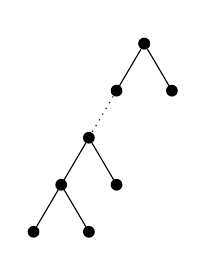
\begin{tikzpicture}[
baseline=-15, scale=1, every node/.style={dotA},
level distance=17pt,
sibling distance=20pt,
]
\node  [label=above:{}]  (root) {}
child {
	child 
	{
		edge from parent[draw=none]
		child 
			{
			child  
			child
			}  
		child
	} 
	child
	{edge from parent[draw=none]}
}
child {};
\node at (root) {};
\node  at (root-1) {};
\node  at (root-2) {};
\node at (root-1-1) {};
\node at (root-1-1-2) {};
\node at (root-1-1-1-2) {};
\node  at (root-1-1-1-1) {};
\node 
at (root-1-1-1) {};
\path  (root-1) edge [ dotted, color=black] (root-1-1) ;
\end{tikzpicture}
\caption{Types $\II$-$\III$.}
\end{subfigure}
\begin{subfigure}[b]{0.2\textwidth}
\centering
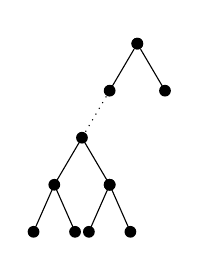
\begin{tikzpicture}[
baseline=-15, scale=1, every node/.style={dotA},
level distance=17pt,
sibling distance=20pt,
level 4/.style={sibling distance=15 pt}
]
\node  [label=above:{}]  (root) {}
child {
	child 
	{
		edge from parent[draw=none]
		child 
			{
			child  
			child
			}  
		child
			{
			child  
			child
			}  
	} 
	child
	{edge from parent[draw=none]}
}
child {};
\node at (root) {};
\node  at (root-1) {};
\node  at (root-2) {};
\path  (root-1) edge [ dotted, color=black] (root-1-1) ;
\node 
at (root-1-1) {};
\node at (root-1-1-2) {};
\node at (root-1-1-1-2) {};
\node  at (root-1-1-1-1) {};
\node at (root-1-1-2-2) {};
\node  at (root-1-1-2-1) {};
\node 
at (root-1-1-1) {};
\node at (root-1-1-2) {};
\end{tikzpicture}
\caption{Type $\IV$.}
\end{subfigure}
\label{FIG:types}
\end{figure}


\begin{lemma}
\label{LEM:wint}
Let $w:\R \times \CC\to \R$ be a smooth function and $\NN$ be as in \eqref{NFE1a}.
Then, we have
\begin{align}
\label{wint0a}
\sum_{j=1}^\infty \sum_{\TT\in \Tr_j} \NN\big(\TT; w+
\D[w, w]
\big)
=
\sum_{j=1}^\infty \sum_{\TT\in\Tr_j} \sum_{\ell=2}^5  \NN_\ell(\TT; w),
\end{align}
where the nonlinear contributions are defined via their spatial Fourier transform
\begin{align}
\label{wint0b}
\begin{split}
\Ft_x \big[ \NN_\ell (\TT; w) \big] & =
\Ical \big(\TT, {\mul}_\l(\TT); w \big),\quad \l=1,\dots, 5,
\end{split}
\end{align}
for $\Ical(\TT, m; w)$ as in \eqref{eq:defiI}, 
where the multipliers are given by 
\begin{align}\label{eq:multiplicadores}
    \mul_1(\<1>)&= K\left(\ind_A  \Psi_0(\<1>) - E\Psi_E(\<1>)\right),\\
    \mul_2(\TT)&=(-1)^{j+1} \ind_{A_\star} K_\star\Psi(\star) \bigg( \prod_{\bul \in \TT^0 \setminus\{\star\}}  K_\bul  \ind_{A_\bul^c} \bigg), 
    && \text{if} \quad  \TT^{0,\ff} = \{\star\}, \ \star\neq \emptyset, 
    \\\mul_3(\TT)&=(-1)^{j}E  \ind_{A_\star^c} K_\star\Psi_E(\star) \bigg( \prod_{\bul \in \TT^0 \setminus\{\star\}}  K_\bul  \ind_{A_\bul^c} \bigg), 
    && \text{if} \quad  \TT^{0,\ff} = \{\star\}, \ \star\neq \emptyset, 
    \\
    \mul_4(\TT)&=(-1)^{j}  K_{\pb(\star)}\Psi(\pb(\star)) \bigg( \prod_{\bul \in \TT^0 \setminus\{\pb(\star)\}}  K_\bul  \ind_{A_\bul^c} \bigg),
    &&
    \text{if} \quad  \TT^{0,\ff} = \{\star\},  \ \star\neq \emptyset
    \label{wint0c}
    \\
     \mul_5(\TT)&=(-1)^{j+1}  K_\star\Psi(\star) \bigg( \prod_{\bul \in \TT^0 \setminus\{\star\}}  K_\bul  \ind_{A_\bul^c} \bigg), 
    && \text{if} \quad  \TT^{0,\ff} = \{\star1, \star2\}, 
    \\
    \mul_{\l}(\TT) & = 0, \ \l=1,2,3,4, 5 && \text{otherwise}, 
\end{align}
with $\TT\in \Tr_j$,  $j \ge 1$, and $K$ and $\Psi$ as in \eqref{Kmul} and \eqref{psi-circ}, respectively.
Moreover, for $\l=1,\ldots, 5$, we will refer to the contributions $\NN_\l(\TT) $ as terms of Type $\I,\II,\III,\IV$ and $\5$, respectively. 



\end{lemma}

\begin{proof}

We first note that there is a unique contribution on the l.h.s.\ of \eqref{wint0a} with homogeneity $2$ in $w$, namely $\NN(\<1>;w,w)$. Therefore,
\[
\NN_1(\<1>;w)=\NN(\<1>;w,w),
\]
and the corresponding multiplier is exactly
\[
\mul_1(\<1>)=K\big(\ind_A\Psi_0(\<1>)-E\Psi_E(\<1>)\big),
\]
in agreement with \eqref{eq:multiplicadores}.

Next, let $j\ge 2$ and $\TT\in\Tr_j$. As in the proof of Lemma~2.10 in the KdV paper, we gather all contributions on the l.h.s.\ of \eqref{wint0a} with underlying tree structure $\TT$, that is, all contributions with tree $\TT$ once the occurrences of $\D[w,w]$ are expanded and the colours are forgotten. Writing $C\subseteq \TT^{0,\ff}$ for the set of final parents which are replaced by $\D[w,w]$, we obtain
\begin{align*}
\sum_{C\subseteq \TT^{0,\ff}}
\NN\Big(\TT\overset{C}{\ominus}\<1>;
f_{\bul}=w \ \text{if } \bul\in (\TT\overset{C}{\ominus}\<1>)^\infty\setminus C,\ 
f_{\bul}=\D[w,w] \ \text{if } \bul\in C\Big)
=
\Ical(\TT,\wt{\mul}(\TT);w),
\end{align*}
where
\[
\wt{\mul}(\TT):=
\sum_{C\subseteq \TT^{0,\ff}}
\mul\big(\TT\overset{C}{\ominus}\<1>\big)\prod_{\star\in C}\mulB(\cherry{\star}{}{}).
\]
Using Proposition~\ref{PRO:NFE}, together with
\[
\mulB(\cherry{\star}{}{})=\ind_{A_\star^c}K_\star,
\qquad \star\in \TT^{0,\ff},
\]
and $(\TT\overset{C}{\ominus}\<1>)^0=\TT^0\setminus C$, we may write
\begin{align*}
\wt{\mul}(\TT)
&=
\sum_{C\subseteq \TT^{0,\ff}}
(-1)^{j+1+|C|}
\bigg(\prod_{\bul\in \TT^0}K_\bul\bigg)
\Bigg[
\sum_{\star\in (\TT\overset{C}{\ominus}\<1>)^{0,\ff}}
\big(\ind_{A_\star}\Psi_0(\star)-\ind_{A_\star^c}E\Psi_E(\star)\big)
\prod_{\bul\in \TT^0\setminus (C\cup\{\star\})}\ind_{A_\bul^c}
\\
&\hspace{5.8cm}
-
\bigg(\prod_{\bul\in \TT^0\setminus C}\ind_{A_\bul^c}\bigg)
\sum_{\star\in (\TT\overset{C}{\ominus}\<1>)^0\setminus (\TT\overset{C}{\ominus}\<1>)^{0,\ff}}
\Psi(\star)
\Bigg].
\end{align*}
As in Lemma~2.10 of the KdV paper, we split this expression into three pieces:
\[
\wt{\mul}(\TT)=\wt{\mul}_{\gfrak,0}(\TT)+\wt{\mul}_{\gfrak,E}(\TT)+\wt{\mul}_{\bfrak}(\TT),
\]
where
\begin{align*}
\wt{\mul}_{\gfrak,0}(\TT)
&=
(-1)^{j+1}
\bigg(\prod_{\bul\in \TT^0}K_\bul\bigg)
\sum_{C\subseteq \TT^{0,\ff}}(-1)^{|C|}
\sum_{\star\in (\TT\overset{C}{\ominus}\<1>)^{0,\ff}}
\ind_{A_\star}\Psi_0(\star)
\prod_{\bul\in \TT^0\setminus\{\star\}}\ind_{A_\bul^c},
\\
\wt{\mul}_{\gfrak,E}(\TT)
&=
(-1)^j E
\bigg(\prod_{\bul\in \TT^0}K_\bul\bigg)
\sum_{C\subseteq \TT^{0,\ff}}(-1)^{|C|}
\sum_{\star\in (\TT\overset{C}{\ominus}\<1>)^{0,\ff}}
\ind_{A_\star^c}\Psi_E(\star)
\prod_{\bul\in \TT^0\setminus\{\star\}}\ind_{A_\bul^c},
\\
\wt{\mul}_{\bfrak}(\TT)
&=
(-1)^j
\bigg(\prod_{\bul\in \TT^0}K_\bul\ind_{A_\bul^c}\bigg)
\sum_{C\subseteq \TT^{0,\ff}}(-1)^{|C|}
\sum_{\star\in (\TT\overset{C}{\ominus}\<1>)^0\setminus (\TT\overset{C}{\ominus}\<1>)^{0,\ff}}
\Psi(\star).
\end{align*}

We now simplify the sums in $C$ by inclusion-exclusion, exactly as in the proof of Lemma~2.10 of the KdV paper.

\smallskip

\noi
\underline{\textbf{Step 1}: simplification of $\wt{\mul}_{\bfrak}(\TT)$.}

Fix $\star\in \TT^0\setminus \TT^{0,\ff}$. The inner sum in $C$ is non-zero only if every child of $\star$ belongs to $\TT^{0,\ff}\cup \TT^\infty$; otherwise, one can vary independently the membership in $C$ of a final parent lying strictly below one of the children of $\star$, and the resulting alternating sum vanishes. Thus, only the following two configurations may contribute.

\smallskip

\noi
\underline{\textbf{Case 1}: $(\star1,\star2)\in \TT^{0,\ff}\times \TT^\infty$ or $(\star1,\star2)\in \TT^\infty\times \TT^{0,\ff}$.}

If $(\star1,\star2)\in \TT^{0,\ff}\times \TT^\infty$, then $\star$ belongs to
\[
(\TT\overset{C}{\ominus}\<1>)^0\setminus (\TT\overset{C}{\ominus}\<1>)^{0,\ff}
\]
if and only if $\star1\notin C$. Hence
\begin{align*}
\sum_{\substack{C\subseteq \TT^{0,\ff}\\ \star\in (\TT\overset{C}{\ominus}\<1>)^0\setminus (\TT\overset{C}{\ominus}\<1>)^{0,\ff}}}
(-1)^{|C|}
=
\sum_{C\subseteq \TT^{0,\ff}\setminus\{\star1\}}(-1)^{|C|}
=
\ind_{\TT^{0,\ff}=\{\star1\}}.
\end{align*}
Taking into account the prefactor $(-1)^j$ in $\wt{\mul}_{\bfrak}(\TT)$, this gives the contribution
\[
(-1)^j
\bigg(\prod_{\bul\in \TT^0}K_\bul\ind_{A_\bul^c}\bigg)
\Psi(\star)\ind_{\TT^{0,\ff}=\{\star1\}}.
\]
The case $(\star1,\star2)\in \TT^\infty\times \TT^{0,\ff}$ is identical and yields the analogous term with $\star2$ in place of $\star1$.

\smallskip

\noi
\underline{\textbf{Case 2}: $\star1,\star2\in \TT^{0,\ff}$.}

In this case, $\star$ belongs to
\[
(\TT\overset{C}{\ominus}\<1>)^0\setminus (\TT\overset{C}{\ominus}\<1>)^{0,\ff}
\]
if and only if $C$ contains at most one of $\star1,\star2$. Therefore
\begin{align*}
\sum_{\substack{C\subseteq \TT^{0,\ff}\\ \star\in (\TT\overset{C}{\ominus}\<1>)^0\setminus (\TT\overset{C}{\ominus}\<1>)^{0,\ff}}}
(-1)^{|C|}
&=
\sum_{C\subseteq \TT^{0,\ff}\setminus\{\star1,\star2\}}
\Big[(-1)^{|C|}+(-1)^{|C|+1}+(-1)^{|C|+1}\Big]
\\
&=
-\ind_{\TT^{0,\ff}=\{\star1,\star2\}}.
\end{align*}
Hence
\begin{align}
\label{eq:mulb-nv-adapted}
\wt{\mul}_{\bfrak}(\TT)
=
(-1)^j
\bigg(\prod_{\bul\in \TT^0}K_\bul\ind_{A_\bul^c}\bigg)
\sum_{\star\in \TT^0\setminus \TT^{0,\ff}}
\Psi(\star)
\Big(
\ind_{\TT^{0,\ff}=\{\star1\}}
+\ind_{\TT^{0,\ff}=\{\star2\}}
-\ind_{\TT^{0,\ff}=\{\star1,\star2\}}
\Big).
\end{align}

\smallskip

\noi
\underline{\textbf{Step 2}: simplification of $\wt{\mul}_{\gfrak,0}(\TT)$ and $\wt{\mul}_{\gfrak,E}(\TT)$.}

The same inclusion-exclusion argument applies here. Fix $\star\in \TT^0$. The inner sum is non-zero only in the following situations.

\smallskip

\noi
\underline{\textbf{Case 1}: $\star\in \TT^{0,\ff}$.}

Then $\star\in (\TT\overset{C}{\ominus}\<1>)^{0,\ff}$ if and only if $\star\notin C$, and therefore
\[
\sum_{\substack{C\subseteq \TT^{0,\ff}\\ \star\in (\TT\overset{C}{\ominus}\<1>)^{0,\ff}}}
(-1)^{|C|}
=
\sum_{C\subseteq \TT^{0,\ff}\setminus\{\star\}}(-1)^{|C|}
=
\ind_{\TT^{0,\ff}=\{\star\}}.
\]

\smallskip

\noi
\underline{\textbf{Case 2}: $(\star1,\star2)\in \TT^{0,\ff}\times \TT^\infty$ or $(\star1,\star2)\in \TT^\infty\times \TT^{0,\ff}$.}

If $(\star1,\star2)\in \TT^{0,\ff}\times \TT^\infty$, then $\star\in (\TT\overset{C}{\ominus}\<1>)^{0,\ff}$ if and only if $\star1\in C$, hence
\[
\sum_{\substack{C\subseteq \TT^{0,\ff}\\ \star\in (\TT\overset{C}{\ominus}\<1>)^{0,\ff}}}
(-1)^{|C|}
=
\sum_{C\subseteq \TT^{0,\ff}\setminus\{\star1\}}(-1)^{|C|+1}
=
-\ind_{\TT^{0,\ff}=\{\star1\}}.
\]
The case $(\star1,\star2)\in \TT^\infty\times \TT^{0,\ff}$ is identical and yields
$-\ind_{\TT^{0,\ff}=\{\star2\}}$.

\smallskip

\noi
\underline{\textbf{Case 3}: $\star1,\star2\in \TT^{0,\ff}$.}

Then $\star\in (\TT\overset{C}{\ominus}\<1>)^{0,\ff}$ if and only if $\{\star1,\star2\}\subseteq C$, so
\[
\sum_{\substack{C\subseteq \TT^{0,\ff}\\ \star\in (\TT\overset{C}{\ominus}\<1>)^{0,\ff}}}
(-1)^{|C|}
=
\sum_{C\subseteq \TT^{0,\ff}\setminus\{\star1,\star2\}}(-1)^{|C|+2}
=
\ind_{\TT^{0,\ff}=\{\star1,\star2\}}.
\]

Combining the three cases, we get
\begin{align}
\label{eq:mulg0-nv-adapted}
\wt{\mul}_{\gfrak,0}(\TT)
&=
(-1)^{j+1}
\sum_{\star\in \TT^0}
\ind_{A_\star}K_\star\Psi_0(\star)
\bigg(\prod_{\bul\in \TT^0\setminus\{\star\}}K_\bul\ind_{A_\bul^c}\bigg)
\nonumber\\
&\hspace{2cm}\times
\Big(
\ind_{\TT^{0,\ff}=\{\star\}}
-\ind_{\TT^{0,\ff}=\{\star1\}}
-\ind_{\TT^{0,\ff}=\{\star2\}}
+\ind_{\TT^{0,\ff}=\{\star1,\star2\}}
\Big),
\\
\label{eq:mulgE-nv-adapted}
\wt{\mul}_{\gfrak,E}(\TT)
&=
(-1)^j E
\sum_{\star\in \TT^0}
\ind_{A_\star^c}K_\star\Psi_E(\star)
\bigg(\prod_{\bul\in \TT^0\setminus\{\star\}}K_\bul\ind_{A_\bul^c}\bigg)
\nonumber\\
&\hspace{2cm}\times
\Big(
\ind_{\TT^{0,\ff}=\{\star\}}
-\ind_{\TT^{0,\ff}=\{\star1\}}
-\ind_{\TT^{0,\ff}=\{\star2\}}
+\ind_{\TT^{0,\ff}=\{\star1,\star2\}}
\Big).
\end{align}

\smallskip

\noi
\underline{\textbf{Step 3}: combination of the three pieces.}

We now combine \eqref{eq:mulb-nv-adapted}, \eqref{eq:mulg0-nv-adapted}, and \eqref{eq:mulgE-nv-adapted}, according to the possible shape of $\TT^{0,\ff}$.

\smallskip

\noi
\underline{\textbf{(i)} $\TT^{0,\ff}=\{\star\}$ with $\star\neq \emptyset$.}

Then only the terms $\star$ and $\pb(\star)$ may contribute. Using
\[
\Psi(\star)=\Psi_0(\star)+E\Psi_E(\star),
\]
the contribution at $\star$ becomes
\begin{align*}
&(-1)^{j+1}\ind_{A_\star}K_\star\Psi_0(\star)
\prod_{\bul\in \TT^0\setminus\{\star\}}K_\bul\ind_{A_\bul^c}
+
(-1)^jE\ind_{A_\star^c}K_\star\Psi_E(\star)
\prod_{\bul\in \TT^0\setminus\{\star\}}K_\bul\ind_{A_\bul^c}
\\
&\qquad =
(-1)^{j+1}\ind_{A_\star}K_\star\Psi(\star)
\prod_{\bul\in \TT^0\setminus\{\star\}}K_\bul\ind_{A_\bul^c}
+
(-1)^jE K_\star\Psi_E(\star)
\prod_{\bul\in \TT^0\setminus\{\star\}}K_\bul\ind_{A_\bul^c},
\end{align*}
which is precisely the sum of the Type $\II$ and Type $\III$ multipliers.

On the other hand, the terms at $\pb(\star)$ coming from
\eqref{eq:mulb-nv-adapted}, \eqref{eq:mulg0-nv-adapted}, and \eqref{eq:mulgE-nv-adapted} combine into
\[
(-1)^j K_{\pb(\star)}\Psi(\pb(\star))
\prod_{\bul\in \TT^0\setminus\{\pb(\star)\}}K_\bul\ind_{A_\bul^c},
\]
which is exactly the Type $\IV$ multiplier.

\smallskip

\noi
\underline{\textbf{(ii)} $\TT^{0,\ff}=\{\star1,\star2\}$.}

Then the only non-zero contribution is at $\star$, and summing the three pieces gives
\[
(-1)^{j+1}K_\star\Psi(\star)
\prod_{\bul\in \TT^0\setminus\{\star\}}K_\bul\ind_{A_\bul^c},
\]
which is the Type $\5$ multiplier.

\smallskip

\noi
\underline{\textbf{(iii)} All remaining trees.}

In this case, all alternating sums above vanish, and therefore
\[
\wt{\mul}(\TT)=0.
\]

Hence, for every $\TT\in \Tr_j$, $j\ge 2$, the total contribution with underlying tree $\TT$ is exactly
\[
\sum_{\ell=2}^5 \Ical(\TT,\mul_\ell(\TT);w),
\]
with $\mul_\ell(\TT)$ given in \eqref{eq:multiplicadores}. Summing over all $j\ge 1$ and all $\TT\in \Tr_j$ yields \eqref{wint0a}. This finishes the proof.
\end{proof}



\begin{align}
\label{w2}
\dt w & =  \sum_{j=1}^\infty \sum_{\TT \in \Tr_j} \sum_{\l=2}^5  \NN_\l(\TT;w),
\end{align}
\simao{Outra letra para z!}
If we now set $w$ to be the interaction representation variable of a new unknown $z$,
\begin{align}
\label{z0}
z(t) : = U(-t) w(t),
\end{align}
we find that $z$ satisfies the gauged Novikov-Veselov equation
\begin{align}
\label{z1}\tag{$\mathcal{G}_\delta$-NV}
\dt z 
+ (\partial^3+\overline{\partial}^3)z + E(\overline{\partial}^{-1}\partial^2 + \partial^{-1}\overline{\partial}^2)z
&
= 
\sum_{j=1}^\infty \sum_{\TT \in \Tr_j} \sum_{\l=1}^5  
U(t)
\NN_\l(\TT;U(-t)z)
\\
&
=: 
 \sum_{j=1}^\infty \sum_{\TT \in \Tr_j} \sum_{\l=1}^5  \Ncal_\l(\TT;z)
.
\end{align}




% It is by now a standard fact [CITAR] that the local well-posedness for \eqref{z1} follows from proving that, for some $b>\frac12$ and $b'>b-1$,
% \begin{equation}\label{eq:multi_geral}
% \left\|\mathcal{N}_\ell(\TT; u_1,\dots, u_{j+1})\right\|_{X^{s,b'}} \le C^j\prod_{k=1}^j \|u_k\|_{X^{s,b}},
% \end{equation}
% for all $\TT\in \Tr^j$, $\ell=1,\dots, 5$, and $j\ge 1$. 


\section{Functional setting and multilinear estimates}\label{sec:multi}


We recall the basic definitions of Fourier restrictions spaces \cite{bourg1, bourg2, tao_book}. Given $s,b\in\R$, we define
\begin{equation}
X^{s,b}=\left\{ u\in \S'(\R\times \R^2) : \jap{\tau-\phi(\xi)}^b\jap{\xi}^s  \widehat{u}\in L^2_{\tau,\xi}(\R\times \R^2)\right\},
\end{equation}
endowed with the induced norm. One can also define the local-in-time $X^{s,b}$ space as
\begin{equation}
X^{s,b}_T=\left\{ u\in \mathcal{D}'((0,T)\times \R^2) : u\equiv v\big|_{(0,T)}\mbox{ for some }v\in X^{s,b}  \right\},\quad T>0.
\end{equation}

The main result of this section, which will yield the local well-posedness of the gauged Novikov-Veselov equation \eqref{z1}, is as follows.
\begin{proposition}\label{prop:bourgL2}
Let $s>-1$, $E\in\CC$ with $|E|<1$, $0<\delta\ll 1$ and $T>0$. Given $j \in\N$, $\TT \in \Tr_j$, and $\Ncal_\l(\TT)$, $\l=1,\dots,5$, there exists $b>\frac12$ such that
	\begin{align}\label{eq:bourg_bi_l2}
		\left\|\int_0^t U(t-t') \Ncal_\l(\TT; z_1,\dots, z_{j+1})(t') dt'  \right\|_{X^{s,b}_T}  \le T^{0+} C^j\delta^{(2s+2)(j-3)-1}\prod_{k=1}^{j+1}\|z_k\|_{X^{s,b}_T}
	\end{align}
    for some constant $C>0$ independent of $j$ and $\TT$.
\end{proposition}


In order to prove Proposition \ref{prop:bourgL2}, we resort to frequency-restricted estimates \cite{COS}. For the sake of completeness, we include below the necessary lemmas for quadratic and higher-order terms, respectively.

\begin{lemma}[{\cite[Lemma 3.1]{CLS}}]\label{lem:fre_bi}
Let $s\in\R$. 
Suppose that, for all $\al\in \R$ and $M>1$, there exists $0<\beta<1$, such that one of the following holds:
\begin{enumerate}
    \item[(i)] for all distinct $ k, \l\in\{\emptyset,1,2\}$\footnote{The empty set symbol $\emptyset$ here corresponds to the frequency component $\xi$, without index.}
    and $1<M\lesssim |\alpha|$,
    \begin{equation}\label{eq:frequad}
        \sup_{\xi_k}\int_{\xi=\xi_1+\xi_2}
        \frac{|m_1(\<1>)|^2\jap{\xi}^{2s}}{\jap{\xi_{1}}^{2s}\jap{\xi_{2}}^{2s}}\mathbbm{1}_{|\Phi(\<1>)-\alpha|<M} d\xi_{\l} \lesssim \jap{\alpha}^\beta M^\beta;
    \end{equation}

    
    % \item[(ii)]
    % there exist distinct $k, \l\in\{1,2\}$ such that
    % \begin{equation}\label{eq:frequad2}
    %     \sup_{\xi_k}\int_{\xi=\xi_1+\xi_2}
    %     \frac{|m_1(\<1>)|^2\jap{\xi}^{2s}}{\jap{\xi_{1}}^{2s}\jap{\xi_{2}}^{2s}}\mathbbm{1}_{|\Phi(\<1>)-\alpha|<M} d\xi_{\l}  \lesssim \jap{\alpha} M^\beta;
    % \end{equation}

    
    \item[(ii)] or we have that
    \begin{equation}\label{eq:frequad3}
        \sup_{\xi}\int_{\xi=\xi_1+\xi_2}\frac{|m_1(\<1>)|^2\jap{\xi}^{2s}}{\jap{\xi_{1}}^{2s}\jap{\xi_{2}}^{2s}}\mathbbm{1}_{|\Phi(\<1>)-\alpha|<M} d\xi_{1}  \lesssim \jap{\alpha}^\beta M;
    \end{equation}
\end{enumerate}
Then there exists $b>\frac12$ such that \eqref{eq:bourg_bi_l2} holds for $\ell=1$ and $\TT=\<1>$.
\end{lemma}



\begin{lemma}[{\cite[Lemma 2]{COS}}]\label{lem:fre_tri}
	Let $s\in\R$, $j\ge 1$, $\ell=2,\dots,5$, and $\TT\in \Tr^j$. Suppose that there exists $B\subset \{\emptyset, 1, \ldots, j+1\}$ be a proper non-empty subset, and  $\M_1 , \M_2: \CC^{j} \to \R^+$ be multipliers satisfying
    \begin{align}
    \frac{|m_\ell(\TT)|^2\jap{\xi}^{2s}}{\prod_{k=1}^j\jap{\xi_{k}}^{2s}}
    \les 
    \M_1(\vec\xi) \M_2(\vec\xi),
    \end{align}
    where $\vec\xi=(\xi_1, \ldots, \xi_{j+1})$.
    Then, if there exists $0<\be<1$ such that
    \begin{equation}\label{L2hypo}
    \sup_{\xi_{k\in B}} \int_{\Gamma(\TT)} \mathcal{M}_1 (\vec\xi) \mathbbm{1}_{|\Phi(\TT)-\alpha|<M} d\xi_{j\notin B} + \sup_{\xi_{j\notin B}} \int_{\Gamma(\TT)} \mathcal{M}_2 (\vec\xi) \mathbbm{1}_{|\Phi(\TT)-\alpha|<M} d\xi_{j\in B} \lesssim C^j M^\beta, 
    \end{equation}
    for all $M\ge 1$ and $\al\in\R$, 
    then there exists $b>\frac12$, depending only on $\be$, such that \eqref{eq:bourg_bi_l2} holds.
\end{lemma}
The restriction $\beta<1$ in Lemmas \ref{lem:fre_bi} and \ref{lem:fre_tri} can be improved to $\beta=1$ at the expense of slightly increasing the weight of the largest frequency, as the next useful lemma shows.
		
\begin{lemma}[{\cite[Lemma 3.3]{CLS}}]\label{lem:eta1}
    Let $K:\R^n\times \R^m\times \R\to \R^+$ be a positive measurable function such that, for some $N\in \mathbb{N}$,
    $$
    |K(x,y,M)|\lesssim \max\{1,|x|,|y|\}^N,\quad \forall x\in\R^n,\ y\in \R^m, \ M\in \R.
    $$
    Suppose that
    $$
    \sup_y \int K(x,y,M)\max\{1,|x|,|y|\}^{0+} dx \lesssim M,\quad \mbox{for all }M>1.
    $$
    Then, there exists $0<\beta<1$ such that
    $$
    \sup_y \int K(x,y,M) dx \lesssim M^{\beta},\quad \mbox{for all } M>1.
    $$
\end{lemma}




The next ingredient concerns the geometry of the resonance functions $\Psi(\TT)$ and is the crux of the multilinear estimates \eqref{eq:bourg_bi_l2}. These properties can also be linked with the optimal decay in the Strichartz estimates associated with the Novikov-Veselov equation [CITE].

\simao{Expandir isto num comentário.}

\begin{lemma}\label{lem:prop_resonance}
Fix $|E|<1$ and $k\ge 2$. Consider the mapping $\Theta:\CC^{k}\to \R$
$$
\Theta(\xi_1,\dots, \xi_{k})= \phi(\xi)-\sum_{j=1}^k \phi(\xi_j),\quad \xi=\sum_{j=1}^{k} \xi_j
$$

\noi{\rm (i)} Over the region
\begin{equation}
V=\left\{\vec{\xi}\in \CC^{k} :\  \frac{1}{\delta}<|\xi_1|,\  |\xi_1\pm\xi|>\delta\max\{|\xi_1|, |\xi|\}\right\},
\end{equation}
we have
$$
|\nabla_{\xi_1}\Theta|\ge 2\delta^2\max\{|\xi_1|^2, |\xi|^2\}.
$$


\noi{\rm (ii)} Suppose that
$$
|\xi_1|\ge |\xi_2| \ge |\xi|\ge |\xi_3|\ge \dots \ge |\xi_k|.
$$
There exist $\delta, \delta'>0$, independent of $k$, and a change of coordinates
\begin{align*}
\varphi:U=\{\vec{\xi}\in \CC^{k} :\  \frac{1}{\delta}<|\xi_1|,\  |\xi_1+\xi|<\delta|\xi_1|\} \mapsto B_{\delta'}(0)\times \CC^{k-1}\\ \vec{\xi} \to (q_1, \xi_2, \dots, \xi_k)
\end{align*}
satisfying
\begin{equation}\label{eq:nondeg}
|\det D_{\xi_1}\varphi| \sim |\xi_2|^{-2}
\end{equation}
and
$$
\Theta(\vec{\xi})=|\xi_2|^3\Re q_1^2 - \sum_{j=2}^k \phi(\xi_j)
$$

\end{lemma}
\begin{proof}
A simple computation shows that, over $V$,
$$
|\nabla_\xi (\phi_0(\xi)-\phi_0(\xi_1))| = 3|\xi^2-\xi_1^2|\ge 3\delta^2\max\{|\xi|^2,|\xi_1|^2\},\quad |\nabla_\xi (\phi_E(\xi)-\phi_E(\xi_1))|\lesssim 1.
$$
In particular, since $|\xi_1|>\frac{1}{\delta}$,
$$
|\nabla_{\xi} \Theta|\gtrsim 3\delta^2\max\{|\xi|^2,|\xi_1|^2\} - 1 \gtrsim 2\delta^2\max\{|\xi|^2,|\xi_1|^2\}.
$$

\noi We now prove (ii). Observe that, over $U$, $|\xi_1|\le 2|\xi_2|$ and $\frac{E}{|\xi|^2}<\delta^2$. Define
$$
p_j=\frac{\xi_j}{|\xi_2|},\quad j=\emptyset, 1,\dots, k,
$$
and write
$$
\Theta=|\xi_2|^3\left(\phi_0(p) - \sum_{j=1}^k \phi_0(p_j) - \frac{E}{|\xi_2|^2}\left(\phi_E(p) - \sum_{j=1}^k \phi_E(p_j)\right)\right).
$$
Setting $c=\sum_{j=2}^kp_k=p-p_1$ and $p_1'=c^{\frac12}\left(p_1+\frac{c}{2}\right)$, we observe that, over $U$,  $c\in C:=\{c\in\CC: 1/3<|c|<3\}$ and $|p_1'|<4\delta$. A trivial computation gives
$$
\phi_0(p)-\phi_0(p_1) = 3\Re (p_1')^2.
$$
Next, consider the function $F:\CC^2\times \R\to \R$ defined as
$$
F(p_1', c, \varepsilon) = 3\Re (p_1')^2 - \varepsilon \left(\phi_E(p_1+c) - \phi_E(p_1)\right).
$$
Fix $c_0\in C$. By an application of Morse's lemma with parameters [CITE], there exist $\delta,\delta'>0$ such that, for $|c-c_0| + |\varepsilon|<\delta$, there exists a change of coordinates $\varphi_{c,\varepsilon}:B_{4\delta}(0)\to B_{\delta'}(0)$, $\varphi_{c,\varepsilon}(p_1')=q_1$, such that
$$
F(p_1', c, \epsilon) = \Re q_1^2
$$
and $|\det D^2_{p_1} \varphi_{c,\varepsilon}|\sim 1$. Since $C$ is a compact set, $\delta, \delta'$ can be chosen independently of $c_0$ (and therefore of $k$).

Returning to $\Theta$, we can now write
$$
\Theta = |\xi_2|^3 F\left(p_1', c, \frac{E}{|\xi_2|^2}\right) - \sum_{j=2}^k \phi(\xi_j) =  |\xi_2|^3\Re q_1^2 - \sum_{j=2}^k \phi(\xi_j) 
$$
and the map $\varphi$ which takes $\xi_1$ into $q_1$ satisfies \eqref{eq:nondeg}. The proof is finished.
\end{proof}
\begin{remark}
By trivial permutations, the conclusions of Lemma \ref{lem:prop_resonance} also hold for other pairings of frequencies.
\end{remark}


For convenience, we compile the pointwise estimates for the multipliers $\mul_\ell(\TT)$, $\ell=1,\dots,5$, in Lemma \ref{LEM:wint} in the next lemma, whose proof is immediate.

\begin{lemma}
Given $\xi_1,\xi_2\in\CC$ and $\xi=\xi_1+\xi_2$,
$$
|\Psi_0(\<1>)|\lesssim |\xi\xi_1\xi_2|,\quad  |\Psi_E(\<1>)|\lesssim \min_{j=\emptyset, 1,2}|\xi_j|,\quad |K|\lesssim \frac{1}{|\xi_1||\xi_2|}.
$$
If $|\xi|\gtrsim 1$, then $|\Psi(\<1>)|\lesssim |\xi\xi_1\xi_2|$.
\end{lemma}

\begin{proof}[Proof of Proposition \ref{prop:bourgL2}]
We split the proof into several steps, depending on each type of nonlinear term and on the length of the underlying tree $\TT$.
\medskip

\noi\textit{Step 1. Type I estimate.} The only nontrivial Type $\I$ term is when $\TT=\<1>$. The corresponding multiplier can be controlled as
$$
|\mul_1(\<1>)|\lesssim |\xi|\ind_A + K|\Psi_E(\<1>)|\ind_{A^c} \lesssim |\xi|\ind_A + \frac{\ind_{A^c}}{\max_{\bul\in\{\emptyset, 1, 2\}}|\xi_\bul|}.
$$
Suppose, without loss of generality, that $|\xi_1|\gtrsim |\xi_2|$. 
For the first term, since $|\xi_2|\lesssim 1$ and $|\partial_{\xi_2}\Psi(\<1>)|\gtrsim |\xi|^2$,  we have
$$
\sup_\xi \int_A \frac{|\xi|^2\jap{\xi}^{2s}}{\jap{\xi_1}^{2s}\jap{\xi_2}^{2s}} \ind_{|\Psi(\<1>)-\alpha|<M} d\xi_2 \lesssim \sup_\xi \int_{|\zeta_2|<1/\delta}  \ind_{|\phi-\alpha|<M} d\phi d\zeta_2 \lesssim \delta^{-1}M
$$
and the estimate follows from Lemma \ref{lem:fre_bi}-(ii) together with Lemma \ref{lem:eta1}.

For the second term, 
% if any frequency is $\lesssim 1$, say $\xi_2$, then
% $$
% \sup_\xi \int_A \frac{\jap{\xi}^{2s}}{\jap{\xi_1}^{2s+2}\jap{\xi_2}^{2s}} \ind_{|\Psi(\<1>)-\alpha|<M} d\xi_2 \lesssim 1.
% $$
% Assuming now that all frequencies are large, 
we may assume that $\xi\not\simeq \pm \xi_2$ (if this is not true, then $\xi_1\not\simeq \pm \xi_2$ and the proof follows from switching $\xi$ with $\xi_1$), which implies that $|\partial_{\xi_2}\Psi(\<1>)|\gtrsim |\xi|^2$. Then
$$
\sup_\xi \int \frac{\jap{\xi}^{2s}}{\jap{\xi_1}^{2s+2-}\jap{\xi_2}^{2s}} \ind_{|\Psi(\<1>)-\alpha|<M} d\xi_2 \lesssim \sup_\xi \int \frac{1}{|\zeta_2|^{4+2s-}} \ind_{|\phi-\alpha|<M}d\phi d\zeta_2 \lesssim M
$$
and we apply once again Lemmas \ref{lem:fre_bi}-(ii) and \ref{lem:eta1}. This concludes the proof for type $\I$ terms.

\medskip

From now on, the proof of \eqref{eq:bourg_bi_l2} for $\ell=2,\dots, 5$ follows from Lemma \ref{lem:fre_tri}, with an appropriate choice of set $B$, and Lemma \ref{lem:eta1}.

\medskip

\noi\textit{Step 2. Type II estimate.} For $\TT\in \Tr_j$, $j\ge 2$,
$$
|\mul_2(\TT)| \lesssim \frac{\jap{\xi}^s}{\jap{\xi_{\star1}}^{s}\jap{\xi_{\star2}}^{s}\jap{\xi_{\sbf(\star)}}^{s+1}}\prod_{\substack{\bul\in\TT^0\\\bul\neq \star, \pb(\star)}} \frac{1}{\jap{\xi_{\bul1}}\jap{\xi_{\bul2}}^{s+1}}.
$$
As we are in $A_\star$, we can assume that $|\xi_{\star2}|\lesssim 1$. Concerning the other frequencies, the worst-case scenario occurs when $\xi_{\star1}$ corresponds to the largest frequency\footnote{We can suppose this because we are not going to use the specific tree structure any further.}. Then, for $\xi$ and $\xi_{\bul2}$, $\bul\in \TT^0\setminus\{\star1\}$, fixed,
\begin{equation}
\int |\xi_{\star1}|^2\ind_{|\Psi(\TT)-\alpha|<M} d\xi_{\star2} \lesssim \int \ind_{|\phi-\alpha|<M} d\phi d\zeta_{\star2} \lesssim M.
\end{equation}
On the other hand, for $\xi_{\star1}. \xi_{\star2}$ fixed, we do not make any use of the resonance restriction:
\begin{align*}
&\int \frac{\jap{\xi}^{2s}}{\jap{\xi_{\star1}}^{2s+2-}\jap{\xi_{\sbf(\star)}}^{2s+2}}\cdot\prod_{\substack{\bul\in\TT^0\\\bul\neq \star, \pb(\star)}} \frac{d\xi_{\bul2}}{\jap{\xi_{\bul1}}^2\jap{\xi_{\bul2}}^{2s+2}}\cdot \ind_{|\Psi(\TT)-\alpha|<M} d\xi\\\lesssim & \int\left(\int \frac{\jap{\xi}^{2s}d\xi}{\jap{\xi_{\star1}}^{2s+2-}\jap{\xi_{\sbf(\star)}}^{2s+2}}\right)\prod_{\substack{\bul\in\TT^0\\\bul\neq \star, \pb(\star)}} \frac{d\xi_{\bul2}}{\jap{\xi_{\bul1}}^2\jap{\xi_{\bul2}}^{2s+2}} \lesssim \delta^{(2s+2)(j-2)}.
\end{align*}


\medskip

\noi \textit{Step 3. Type IV estimate, $j=2$.} It is convenient to consider the case $\pb(\star)=\emptyset$ separately. If so, then we can assume that $\TT=\<21>$ and 
\begin{equation}
\label{typeIVmult2}
|\mul_4(\TT)|\lesssim \frac{\jap{\xi}^{s+1}}{\jap{\xi_{11}}^{s+1}\jap{\xi_{12}}^{s+1}\jap{\xi_2}^s}.
\end{equation}
The worst-case scenario corresponds to $|\xi_2|\ge |\xi|\ge |\xi_{11}|\ge |\xi_{12}|$. The proof follows deriving bounds on
\begin{equation}\label{eq:type4interp1}
\sup_{\xi,\xi_{12},\alpha} \int |\xi|^{1-} \ind_{|\Psi(\TT)-\alpha|<M}d\xi_{11}
\end{equation}
and
\begin{equation}\label{eq:type4interp2}
\sup_{\xi_2,\xi_{11},\alpha} \int \frac{|\xi|^{1+}}{\jap{\xi_{12}}^{4s+4}}\ind_{|\Psi(\TT)-\alpha|<M}d\xi_{12}
\end{equation}

\smallskip
\noi\textbf{Case A.} $\xi\not\simeq \pm \xi_{12}$ and $\xi_2\not\simeq \pm \xi_{11}$.

\noi For $\xi, \xi_{12}$ fixed, we bound
\begin{equation}\label{eq:typeIVest1}
\eqref{eq:type4interp1}\lesssim \int \frac{1}{|\xi_2|^{1+}}\ind_{|\phi-\alpha|<M}d\phi d\zeta_{11} \lesssim M.
\end{equation}
For $\xi_2, \xi_{11}$ fixed,
\begin{equation}\label{eq:typeIVest2}
\eqref{eq:type4interp2} \lesssim \int \frac{1}{\jap{\xi_{12}}^{4s+4}|\xi|^{1-}}\ind_{|\Psi(\TT)-\alpha|<M}d\phi d\zeta_{12} \lesssim M.
\end{equation}

\smallskip
\noi
\textbf{Case B.} $\xi\simeq \pm \xi_{12}$ or $\xi_2\simeq \pm \xi_{11}$. Observe that this implies that all frequencies are comparable and thus
$$
|\mul_4(\TT)|\lesssim |\xi|^{-1-2s}.
$$

\smallskip
\noi
\textbf{Case B1.} Up to permutations, the conditions of Case A are met. It suffices to follow the arguments therein.

\smallskip
\noi
\textbf{Case B2.} We have three frequencies which are equal (up to a sign), say $\xi_2\simeq  \xi_{11} \simeq \pm \xi_{12}$. If the sign is the same, then
$$
\xi_2\simeq \xi_{11}\simeq \xi_{12} \simeq \frac{\xi}{3}.
$$
For $\xi_2, \xi_{11}$ fixed, we proceed as in Case A (since the nonstationary condition is still satisfied). For $\xi, \xi_{12}$ fixed, we apply Lemma \ref{lem:prop_resonance}-(ii) to estimate
\begin{align}
\eqref{eq:type4interp1}\lesssim \int_{|q_1|\ll 1} |\xi_2|^{3-}\ind_{||\xi|^3\Re q_1^2 - \Tilde{\alpha}|<M} dq_1 \lesssim M^{1^-}
\end{align}

% For $\xi_2, \xi_{11}$ fixed, we proceed as in \eqref{eq:typeIVest2}. For $\xi, \xi_{12}$ fixed, we define
% $$
% p_\bul = \frac{\xi_\bul}{|\xi|}, \qquad\bul=\emptyset, 2, 11, 12.
% $$
% The resonance function can be written as
% $$
% \Psi(\TT)=|\xi|^3 \left(P(p_2)-\frac{E}{|\xi|^2}R(p_2)\right),\quad P(p_2)=\Re(p^3-p_2^3-p_{11}^3-p_{12}^3)
% $$
% $$
% R(p_2)=\Re\left(p^3-\frac{p_2^3}{|p_2|
% ^2}-\frac{p_{11}^3}{|p_{11}|^2}-\frac{p_{12}^3}{|p_{12}|^2}\right) 
% $$
% Consider the function
% $$
% F(p_2;p, p_{12}, \varepsilon)= P(p_2) + \varepsilon R(p_2)
% $$
% For $\epsilon =0$, we are near a nondegenerate stationary point $p_2^0$ of $F$. Then, by Morse's lemma with parameters, for $\varepsilon>0$ small, there exist $\lambda_1, \lambda_2\in \{\pm1\}$ such that
% $$
% F(p_2;p, p_{12}, \varepsilon) = c(p, p_{12}, \varepsilon) + \lambda_1 q_2^2 + \lambda_2 r_2^2, \quad q_2,r_2\in \R, \quad |q_2|+|r_2|\ll 1.
% $$
% Then, for $\epsilon=-E/|\xi|^2$, we bound 
% \begin{align*}
% \eqref{eq:type4interp2}\lesssim &\int |\xi|^{3-} \ind_{|\Psi(\TT)-\alpha|<M}dp_{2}\\\lesssim &\int_{|q_2|+|r_2|\ll 1}|\xi|^{3-} \ind_{|c(p, p_{12}, \varepsilon) + \lambda_1 q_2^2 + \lambda_2 r_2^2-\alpha|<M}dq_{2}dr_2 \lesssim M^{1-}
% \end{align*}

Finally, if $\xi_2\simeq \xi_{11}\simeq-\xi_{12}$, then $\xi\simeq -\xi_{12}$. In this case, in both \eqref{eq:type4interp1} and \eqref{eq:type4interp2}, we proceed using Lemma \ref{lem:prop_resonance}-(ii) as above.

\medskip

\noi \textit{Step 4. Type IV estimate, $j\ge3$.}
Denote $\circ=\gb(\star)$. Then
\begin{equation}\label{eq:typeIVmult}
|\mul_4(\TT)|\lesssim \frac{\jap{\xi}^{s}}{\jap{\xi_{\circ111}}^{s+1}\jap{\xi_{\circ112}}^{s+1}\jap{\xi_{\circ12}}^{s}\jap{\xi_{\circ2}}^{s+1}} \prod_{\bul\in\TT^\infty, \bul\ngeq\circ} \frac{1}{\jap{\xi_\bul}^{s+1}\jap{\xi_{\sbf(\bul)}}}
\end{equation}
We focus on the worst-case scenario $|\xi_{\circ12}|\ge |\xi_{\circ 2}|\ge |\xi_{\circ 111}| \ge |\xi_{\circ 112}| \ge |\xi|$. We then consider the quantities
\begin{equation}\label{eq:IVinterp1}
\sup_{\xi_{\circ111}, \xi_{\circ12}}\int \frac{\jap{\xi}^{2s}}{|\xi_{\circ12}|^{1+2s}}\left(\prod_{\bul\in\TT^\infty, \bul\ngeq\circ} \frac{d\xi_\bul}{\jap{\xi_\bul}^{2s+2}\jap{\xi_{\sbf(\bul)}}^2}\right) \ind_{|\Psi(\TT)-\alpha|<M}d\xi d\xi_{\circ112}
\end{equation}
and
\begin{equation}\label{eq:IVinterp2}
\sup_{\xi, \xi_{\circ2}, \xi_{\circ112}, \xi_{\bul\in\TT^\infty, \bul\ngeq\circ}, }\int \frac{|\xi_{\circ12}|^{1+}}{\jap{\xi_{\circ111}}^{2s+2}\jap{\xi_{\circ112}}^{2s+2}\jap{\xi_{\circ2}}^{2s+2}}\ind_{|\Psi(\TT)-\alpha|<M} d\xi_{\circ111}
\end{equation}

\smallskip
\noi\textbf{Case A.} $\xi_{\circ12}\not\simeq \pm \xi_{\circ111}$ and $\xi_{\circ2}\not\simeq \pm \xi_{\circ112}$.

\noi For $\xi_{\circ12}, \xi_{\circ111}$ fixed, we estimate
\begin{align*}
\eqref{eq:IVinterp1}\lesssim & \int \frac{\jap{\xi}^{2s}}{|\xi_{\circ12}|^{3+2s}}\left(\prod_{\bul\in\TT^\infty, \bul\ngeq\circ} \frac{d\xi_\bul}{\jap{\xi_\bul}^{2s+2}\jap{\xi_{\sbf(\bul)}}^2}\right) \ind_{|\phi-\alpha|<M}d\xi d\zeta_{\circ112}\lesssim \delta^{(2s+2)(j-3)}M
\end{align*}
while, for $\xi, \xi_{\circ2}, \xi_{\circ112}$ and $\xi_{\bul\in \TT^\infty, \bul\ngeq \circ}$ fixed, we bound
\begin{align*}
\eqref{eq:IVinterp2} \lesssim & \int \frac{1}{\jap{\xi_{\circ111}}^{2s+2}|\xi_{\circ2}|^{1-}}\ind_{|\Psi(\TT)-\alpha|<M} d\phi d\zeta_{\circ111} \lesssim M
\end{align*}

\smallskip
\noi
\textbf{Case B.} $\xi_{\circ12}\simeq \pm \xi_{\circ111}$ or $\xi_{\circ2}\simeq \pm \xi_{\circ112}$.

\noi It suffices to proceed as in the corresponding Case B in Step 3, applying if necessary the change of coordinates of Lemma \ref{lem:prop_resonance}-(ii). We leave the details to the interested reader.


\smallskip
\noi\textit{Step 5. Type III estimate.} Given $\TT\in \Tr_j$, $j\ge 2$, since $|\Psi_E(\star)|\lesssim |\xi_\star|$,
$$
|\mul_3(\TT)|\lesssim \frac{\jap{\xi}^{s}}{\jap{\xi_{\star1}}^{s+1}\jap{\xi_{\star2}}^{s+1}\jap{\xi_{\sbf(\star)}}^{s+1}}\prod_{\bul \in \TT^\infty, \bul\ngeq \pb(\star)}\frac{1}{\jap{\xi_{\bul}}\jap{\xi_{\sbf(\bul)}}^{s+1}}
$$
If $j=2$, this is a stronger bound than \eqref{typeIVmult2}.
If $j\ge 3$, taking $\circ=\gb(\star)$, this estimate can be rewritten as
$$
|\mul_3(\TT)|\lesssim \frac{\jap{\xi}^s}{\jap{\xi_{\circ111}}^{s+1}\jap{\xi_{\circ112}}^{s+1}\jap{\xi_{\circ12}}^{s+1}\jap{\xi_{\circ1}}\jap{\xi_{\circ2}}^{s+1}} \prod_{\bul \in \TT^\infty, \bul\ngeq \circ}\frac{1}{\jap{\xi_{\bul}}\jap{\xi_{\sbf(\bul)}}^{s+1}}
$$
which is smaller than the bound in \eqref{eq:typeIVmult}. In any case, the estimate for type $\III$ terms is reducible to that for type $\IV$.



% If $|\xi_\star|\lesssim |\xi_{\pb(\star)}|$, then this can be controlled as in Type $\IV$ terms. We therefore assume that $|\xi_\star|\gg |\xi_{\pb(\star)}|$, which implies that $\xi_{\star1}+\xi_{\star2}\simeq -\xi_{\sbf(\star)}$. Assuming, without loss of generality, that $|\xi_{\star1}|\ge |\xi_{\star2}|\ge |\xi_{\sbf(\star)}|$, we must have $\xi_{\sbf(\star)}\not\simeq \pm \xi_{\star1}$. Moreover, the worst-case scenario occurs when all three frequencies are $\gtrsim |\xi|$.

% For $\xi_{\star1}, \xi_{\star2}, \xi_{\sbf(\star)}$ fixed,
% $$
% \int \frac{\jap{\xi}^{2s}}{|\xi_{\star1}|^{2s+2}}\left(\prod_{\bul\in\TT^\infty, \bul\ngeq \pb(\star)} \frac{d\xi_\bul}{\jap{\xi_{\sbf(\bul)}}^2\jap{\xi_\bul}^{2s+2}}\right)d\xi \lesssim \delta^{(2s+2)j}.
% $$
% On the other hand, given $\xi, \xi_{\bul\in \TT^\infty, \bul\ngeq \pb(\star)}$,
% $$
% \int \frac{1}{\jap{\xi_{\star2}}^{2s+2}\jap{\xi_{\sbf(\star)}}^{2s+2}}\ind_{|\Psi(\TT)-\alpha|<M}d\xi_{\star2}d\xi_{\sbf(\star)}
% $$


\medskip
\noi\textit{Step 6. Type V estimate, $j=3$.} Once again, we must consider the case $\star=\emptyset$ separately. In this situation, $\TT=\<33>$ and the corresponding multiplier can be controlled as
$$
|\mul_5(\TT)|\lesssim \frac{\jap{\xi}^{s+1}}{\jap{\xi_{11}}^{s+1}\jap{\xi_{12}}^{s+1}\jap{\xi_{21}}^{s+1}\jap{\xi_{22}}^{s+1}}
$$
The worst-case scenario occurs when $|\xi|\ge |\xi_{11}|\ge |\xi_{12}|\ge |\xi_{21}|\ge |\xi_{22}|$ and we consider the quantities
\begin{equation}\label{eq:Vinterp1}
\sup_{\xi, \xi_{12}, \xi_{22}}\int |\xi|^{1-} \ind_{|\Psi(\TT)-\alpha|<M} d\xi_{21}
\end{equation}
and
\begin{equation}\label{eq:Vinterp2}
\sup_{\xi_{11}, \xi_{21}}\int \frac{1}{|\xi|^{1-}\jap{\xi_{12}}^{2s+2}\jap{\xi_{21}}^{2s+2}\jap{\xi_{22}}^{2s+2}}\ind_{|\Psi(\TT)-\alpha|<M} d\xi_{12}d\xi_{22}.
\end{equation}

\smallskip
\noi\textbf{Case A.} $\xi\not\simeq \pm \xi_{12}$ and $\xi_{11}\not\simeq \pm\xi_{21}$.

\noi For $\xi, \xi_{12}, \xi_{22}$ fixed,
\begin{equation}\label{eq:estVinterp1}
\eqref{eq:Vinterp1} \lesssim \int \frac{1}{|\xi|^{1+}} \ind_{|\phi-\alpha|<M} d\phi  d\zeta_{21} \lesssim M 
\end{equation}
and, for $\xi_{11}, \xi_{21}$ fixed,
\begin{equation}\label{eq:estVinterp2}
\eqref{eq:Vinterp2} \lesssim \int \frac{1}{|\xi_{11}|^{1-}\jap{\zeta_{12}}^{2s+2}\jap{\xi_{22}}^{4s+4}} \ind_{|\phi-\alpha|<M}  d\phi d\zeta_{21}d\xi_{22} \lesssim M.
\end{equation}

\smallskip
\noi\textbf{Case B.} $\xi\simeq \pm \xi_{12}$ or $\xi_{11}\simeq \pm\xi_{21}$. This implies in particular that $|\xi|\sim |\xi_{21}|$.
We split further into two cases:

\smallskip
\noi\textbf{Case B1.} Up to permutations of $\xi, \xi_{11}, \xi_{12}$ and $\xi_{21}$, the conditions of Case A are met (in which case we proceed as above).

\smallskip
\noi\textbf{Case B2.} The frequencies $\xi_{11}, \xi_{12}$ and $\xi_{21}$ are equal up to a sign. In this case, up to permutation of the frequencies, we can suppose that
$$
\xi \not\simeq \xi_{12} \quad \mbox{and}\quad \xi_{11}\not\simeq -\xi_{21}.
$$
For $\xi, \xi_{12}, \xi_{22}$ fixed, either $\xi_{11} \not\simeq -\xi_{31}$ (and we bound \eqref{eq:Vinterp1} as in \eqref{eq:estVinterp1}) or $\xi_{11}\simeq -\xi_{31}$. In the latter case, by Lemma \ref{lem:prop_resonance}-(ii),
\begin{equation}
\eqref{eq:Vinterp1} \lesssim \int |\xi|^{3-}\ind_{||\xi|^2\Re q_1^2 - \Tilde{\alpha}|<M} dq_1 \lesssim M^{1-}.
\end{equation}
For $\xi_{11}, \xi_{21}$ fixed, we split analogously in the nonstationary and stationary cases, arguing as in \eqref{eq:estVinterp2} or using Lemma \ref{lem:prop_resonance}-(ii).

\medskip
\noi\textit{Step 7. Type V estimate, $j\ge 4$.} In this case,  the multiplier can be controlled as
$$
|\mul_5(\TT)| \lesssim \frac{\jap{\xi}^s}{\jap{\xi_{\star11}}^{s+1}\jap{\xi_{\star12}}^{s+1}\jap{\xi_{\star21}}^{s+1}\jap{\xi_{\star22}}^{s+1}\jap{\xi_{\sbf(\star)}}^{s+1}} \prod_{\bul \in \TT^\infty, \bul\ngeq \pb(\star)} \frac{1}{\jap{\xi_{\sbf(\bul)}}\jap{\xi_\bul}^{s+1}}
$$
In the worst-case scenario, $|\xi_{\star11}|\ge|\xi_{\star12}|\ge|\xi_{\star21}|\ge|\xi_{\star22}|\ge|\xi_{\sbf(\star)}|\ge |\xi|$. We consider
\begin{equation}\label{eq:Vinterp3}
\sup_{\xi_{\star11}, \xi_{\star21}, \xi_{\sbf(\star)}} \int \frac{\jap{\xi}^{2s}}{|\xi_{\star11}|^{1+2s}}\prod_{\bul \in \TT^\infty, \bul\ngeq \pb(\star)} \frac{d\xi_\bul}{\jap{\xi_{\sbf(\bul)}}^2\jap{\xi_\bul}^{2s+2}}\ind_{|\Psi(\TT)-\alpha|<M}d\xi d\xi_{\star22}
\end{equation}
and
\begin{equation}\label{eq:Vinterp4}
\sup_{\xi, \xi_{\star12}, \xi_{\star22}, \xi_{\bul \in \TT^\infty, \bul\ngeq \pb(\star)}} \int \frac{1}{|\xi_{\star11}|^{1-}\jap{\xi_{\star21}}^{4s+4}\jap{\xi_{\sbf(\star)}}^{4s+4}} \ind_{|\Psi(\TT)-\alpha|<M} d\xi_{\star21}d\xi_{\sbf(\star)}.
\end{equation}
Notice that \eqref{eq:Vinterp3} corresponds to \eqref{eq:IVinterp1}, while \eqref{eq:Vinterp4} is similar to\eqref{eq:IVinterp2}, with the exception that it has an extra integration and an extra $|\xi_{\star11}|^2$ weight to compensate. It now suffices to proceed as in Step 4.
\end{proof}

\section{Proof of the main theorem}

In this section, we prove Theorem \ref{thm:main_intro}. By a suitable rescaling, it suffices to consider the case $|E|<1$. Throughout this section, we fix $R\gg 1$ and take $\delta>0$ such that
\begin{equation}\label{eq:escolhadelta}
\delta^{2s+2}R\ll 1.
\end{equation}

\begin{proposition}[Local well-posedness for the gauged NV equation]\label{prop:lwp_rnv}
Fix $s>-1$. Given $z_0\in H^s(\R^2)$ with $\|z_0\|_{H^s}<R$, there exist $T=T_{\delta,R}>0$ and a unique
$$
z\in X^{s,\frac12 +}(0,T)
$$
solution of \eqref{z1} over $(0,T)$ with initial data $z_0$.
\end{proposition}

\begin{proof}
While the proof is standard, we sketch the main estimates to highlight the dependence on $\delta$.

Fix $b=\frac12+$. Define 
$$
B_{R,T}=\left\{ z\in X^{s,b} : \|z\|_{X^{s,b}(0,T)}\le 2R \right\},
$$
endowed with the induced distance, and
$$
\Theta[z](t)=U(t)z_0 + \int_0^t U(t-t')\sum_{j=1}^\infty \sum_{\TT \in \Tr_j} \sum_{\l=1}^5  \Ncal_\l(\TT;z)(t')dt'
$$
Applying the multilinear estimates in Proposition \ref{prop:bourgL2}, given $z\in B_{R,T}$,
\begin{align}
\|\Theta[z]\|_{X^{s,b}(0,T)} &\le \|z_0\|_{H^s} + T^{0+}\sum_{j=1}^\infty \sum_{\TT \in \Tr_j} \sum_{\l=1}^5 C^j\delta^{(2s+2)(j-3)-1}\|z\|_{X^{s,b}(0,T)}^{j+1} \\&\le R + T^{0+}\sum_{j=1}^\infty C^j\delta^{(2s+2)(j-3)-1}R^{j+1} \\&\le R+T^{0+}C\delta^{-4s-5}R^2 \le 2R,
\end{align}
for $T=T_{\delta,R}$ sufficiently small. Using the multilinear structure of the nonlinear terms, an analogous computation yields
$$
\|\Theta[z]-\Theta[z']\|_{X^{s,b}(0,T)} \le T^{0+}C\delta^{-4s-5}R\|z-z'\|_{X^{s,b}(0,T)} \le \frac12\|z-z'\|_{X^{s,b}(0,T)}.
$$
The result now follows from Banach's fixed point theorem.
\end{proof}

\begin{remark}\label{remark:persistence}
If $z_0\in H^{s'}(\R^2)$, for some $s'>s$, a standard persistence-of-regularity argument shows that $z\in X^{s',b}(0,T) \hookrightarrow C([0,T]; H^s(\R^2))$.
\end{remark}


Recall the (formal) definition of the gauge transform,
\begin{equation}\label{eq:gauge}
\mathcal{G}_\delta^{-1}[f]=f+\F_{z}^{-1}\left(\int_{\xi=\xi_1+\xi_2} K\mathbbm{1}_{A^c_\delta}(\xi_1,\xi_2)\widehat{f}(\xi_1)\widehat{f}(\xi_2)d\xi_1\right).
\end{equation}



\begin{lemma}\label{LEM:D}

Consider the map  $\Gc^{-1}$ defined in \eqref{eq:gauge}.

\smallskip



\noi {\rm(i)}
Let $s' \ge s>-1$, $R>0$, $0<\dl \ll R^{-\frac{1}{2s+2}}$, and $B_{R}^{s',s}$ given by
\begin{align}
\label{Bss}
B^{s',s}_\delta=\left\{ f\in H^{s'}(\R^2): \|f\|_{H^s} \le R \right\}.
\end{align}
Then, there exists $0<\epsilon\ll 1$ such that the map $\Gc_\dl^{-1}: B^{s, s'}_R \to B^{s,s'}_{(1+\eps)R}$ is continuous with a continuous inverse $\Gc_\dl: B^{s',s}_{(1-\eps)R} \to B^{s',s}_R$.

\smallskip
\noi {\rm(ii)} The map $\Gc_\dl^{-1}$ is unbounded on $H^s(\R^2)$ for $s< - 1$.


\end{lemma}

\begin{proof}
We start with (i). It suffices to check that the quadratic term in \eqref{eq:gauge} is a (small) bilinear map over $B_R$. Supposing, without loss in generality, that $|\xi|\le |\xi_1|\sim |\xi_2|$,
\begin{align*}
&\sup_{\|g\|_{L^2}\le 1} \int_{\xi=\xi_1+\xi_2} \jap{\xi}^sK\mathbbm{1}_{A^c_\delta}(\xi_1,\xi_2)\widehat{f}_1(\xi_1)\widehat{f}_2(\xi_2)g(\xi)d\xi_1d\xi \\\lesssim & \sup_{\xi_1} \left(\int_{\xi=\xi_1+\xi_2} \mathbbm{1}_{A^c_\delta} \frac{\jap{\xi}^{2s}}{\jap{\xi_1}^{2s+2}\jap{\xi_2}^{2s+2}}d\xi\right)^{\frac12}\|f_1\|_{H^s}\|f_2\|_{H^s} \lesssim \delta^{2+2s}\|f_1\|_{H^s}\|f_2\|_{H^s},
\end{align*}
and the claim follows from \eqref{eq:escolhadelta}.

To prove (ii), take $\widehat{f}(\xi)=\jap{\xi}^{-1-s-}$. Then, for $|\xi|<1$,
$$
\int_{\xi=\xi_1+\xi_2} K\ind_{A^c_\dl}(\xi_1,\xi_2)\widehat{f}(\xi_1)\widehat{f}(\xi_2)d\xi_1 \sim \int \frac{1}{\jap{\xi_1}^{4+2s+}}d\xi_1 = \infty,
$$
since $s<-1$.
\end{proof}

\simao{For $s=-1$, the gauge transform is still a bounded operator: in dual form, we must prove that
$$
\left|\int_{\xi=\xi_1+\xi_2} \ind_{A^c}\frac{\widehat{f}(\xi_1)\widehat{f}(\xi_2)\widehat{g}(\xi)}{\jap{\xi}} d\xi_1d\xi\right|\lesssim \|f\|_{L^2}^2\|g\|_{L^2}
$$
which is is a consequence of
$$
\left|\int \jap{\dx}^{-1}h g dx\right|\lesssim \|h\|_{L^1}\|g\|_{L^2},\quad (h=(\mathbf{P}_{>1}f)^2),
$$
and thus reducible to
$$
\|h\|_{L^2(\R^2)}\lesssim \|h\|_{W^{1,1}(\R^2)},
$$
the endpoint of Sobolev embedding (which holds nevertheless). 
}

To conclude the proof of Theorem \ref{thm:main_intro}, we proceed via a density argument as in the KdV case \cite{chcora}, which hinges on the following equivalence result.

\begin{proposition}\label{PRO:equiv}
Let $s' \ge s > -1$ with $s'\gg1$ sufficiently large, $R>0$, $0<\dl \ll R^{-\frac{1}{2s+2}}$, and $u_0$ satisfying
\begin{align}
\label{equiv-0}
u_0\in H^{s'}(\R)
\quad
\text{and}
\quad
 \|u_0\|_{H^s}<R.
\end{align}
Moreover, let $u \in X^{s',b}(0,T)$ be the solution to \eqref{eq:NV} with initial data $u_0$, for some $T>0$, constructed in
\cite{angelopolous, kazeykinamunoz1, kazeykinamunoz2}, and $z\in X^{s', b}(0,T_{\delta,R})$ be the solution to \eqref{z1}
 with initial data $z_0 := \Gc_\delta[u_0]$ in Proposition~\ref{prop:lwp_rnv}.
Then, we must have $T \ge T_{\delta,R}$ and the following identity holds:
\begin{align} \label{equiv-1}
z(t)=\Gc_\delta[u(t)]
\quad
\text{in}
\quad
C([0,T_{\delta,R}]; H^{s'}(\R^2)).
\end{align}
\end{proposition}

\begin{proof}[Sketch of the proof] As the proof follows exactly as in \cite[Section 5]{chcora}, we just give a brief overview of the key ingredients.

\smallskip
First, setting $\widehat{\mathbf{P}_nu}(\xi):=\ind_{[0,n]}(|\xi|)\widehat{u}(\xi)$, one considers the solution $u_n$ of truncated \eqref{eq:NV} equation
\begin{equation}\tag{NV$_n$}\label{eq:NV_n}
	\partial_t u + (\partial^3 + \overline{\partial}^3)u + \frac34\mathbf{P}_n(\partial(u\overline{\partial}^{-1}\partial u) + \overline{\partial}(u\partial^{-1}\overline{\partial}u)) + E(\overline{\partial}^{-1}\partial^2 u + \partial^{-1}\overline{\partial}^2 u)=0,
\end{equation}
with initial data $u_0\in H^s(\R^2)$.
Since the algebraic procedure described in Section \ref{sec:nfe} are independent of $n$, we may also write the corresponding truncated gauged transform via its inverse
\begin{equation}\label{eq:gauge_n}
\mathcal{G}_{\delta,n}^{-1}[f]=f+\F_{z}^{-1}\left(\int_{\xi=\xi_1+\xi_2} K\ind_{[0,n]}(|\xi|)\mathbbm{1}_{A^c_\delta}(\xi_1,\xi_2)\widehat{f}(\xi_1)\widehat{f}(\xi_2)d\xi_1\right),
\end{equation}
and the gauged variable $z_n(t)=\mathcal{G}_{\delta,n}[u_n](t)$ satisfies the corresponding gauged \eqref{eq:NV_n} equation. Observe that Lemma \ref{LEM:D} holds regardless of $n$.

\smallskip
On the other hand, the multilinear estimates (Proposition \ref{prop:bourgL2})  are also independent of $n$. By the proof of Proposition \ref{prop:lwp_rnv} (see also Remark \ref{remark:persistence}), the truncated gauged equation is well-posed in for initial data $z_{0,n}\in H^{s'}(\R)$ with $\|z_{0,n}\|_{H^s}<R$, yielding a solution $z'_{n}\in C([0,T_{\delta,R}]; H^{s'}(\R^2))$ with $\|z_{n}'\|_{L^\infty_tH^s}<2R$. Using the truncation of the nonlinearity onto low frequencies, one then proves that $\mathcal{G}_{\delta,n}[u_n]=z_n=z'_n$ in $C([0,T_{\delta,R}]; H^s(\R^2))$ via uniqueness in\footnote{This is where the Fourier truncation is necessary, as it lets us prove that the two solutions coincide on intervals of size $\sim T/n$.}$L^\infty_tH^s$. Notice in particular that this gives the uniform time-of-existence for the solutions $u_n$, which was not guaranteed by the \eqref{eq:NV} at high regularity \cite{angelopolous, kazeykinamunoz1, kazeykinamunoz2}.

\smallskip
Having shown the equivalence between the truncated equations at high regularity, it remains to prove that, as $n\to \infty$, $u_n$ converges to the \eqref{eq:NV} solution $u$ and $z_n$ converges to the \eqref{z1} solution $z$. This is an easy consequence of the multilinear estimates in $X^{s',b}$. Then, taking the limit in $n$ in the relation $\mathcal{G}_{\delta,n}[u_n]=z_n$, the proof is finished.
\end{proof}

In particular, for smooth data in
$$
B_R=\{u\in H^s(\R^2) : \|u\|_{H^s}< R \},
$$
the \eqref{eq:NV} is conjugate (via $\Gc_{\delta}$) to the \eqref{z1} flow, with a uniform local time of existence. Since both the gauge transform $\Gc_\delta$, its inverse $\Gc_{\dl}^{-1}$, and the \eqref{z1}-flow have continuous (and even analytic) extensions to $B_R$, this concludes the proof of Theorem \ref{thm:main_intro}.



\appendix

\section{Improved local well-posedness for $s>-\frac34$}

In this short appendix, we extend the well-posedness result in $H^s, s>-\frac34,$ of Adams and Grünrock for the zero-energy \eqref{eq:NV} to the nonzero case. In particular, we are able to improve the properties of the \eqref{eq:NV} flow constructed in Theorem \ref{thm:main_intro}. 


\begin{theorem}\label{thm:s-34}
Fix $E\in \R$ and $s>-\frac34$. Given $u_0\in H^s(\R^2)$, there exists $T>0$ and a unique $u\in X^{s,b}_T$ strong integral solution to \eqref{eq:NV} with initial data $u_0$. Moreover, the data-to-solution map is analytic.
\end{theorem}


As before, using the scaling invariance, it suffices to prove Theorem \ref{thm:s-34} for $|E|<1$. We define the bilinear operator associated with the \eqref{eq:NV} nonlinearity (see \eqref{eq:NV2}):
$$
B[u_1,u_2]^\wedge(\xi):=\int_{\xi=\xi_1+\xi_2} K\Phi_0u_1(\xi_1)u_2(\xi_2)d\xi_1
$$
Then, using the standard theory of Fourier restriction norm spaces (\cite{bourg1,bourg2}, see also the monographs \cite{linaresponce, tao_book}), the proof of Theorem \ref{thm:s-34} follows from 

\begin{proposition}
Fix $E\in \R$ and $s>-\frac34$. Then
\begin{equation}\label{eq:bilin_s-34}
\left\| B[u_1,u_2]\right\|_{X^{s,-\frac12+}}\lesssim \|u_1\|_{X^{s,\frac12+}}\|u_2\|_{X^{s,\frac12+}}
\end{equation}

\end{proposition}

\begin{proof}
First, we decompose $B$ as
\begin{align*}
B[u_1,u_2]^\wedge(\xi)&=\int_{\xi=\xi_1+\xi_2} K\Phi\mathbbm{1}_{A^c}u_1(\xi_1)u_2(\xi_2)d\xi_1 \\&\qquad+ \int_{\xi=\xi_1+\xi_2} K(\Phi_0\mathbbm{1}_A -E\Phi_E\mathbbm{1}_{A^c})u_1(\xi_1)u_2(\xi_2)d\xi_1
\end{align*}
The bilinear estimate for the last term as already been shown in Proposition \ref{prop:bourgL2} (it corresponds to the type $\I$ term). For the remaining term, we will use Lemma \ref{lem:fre_bi}-(i) (together with Lemma \ref{lem:eta1}) and prove the necessary frequency-restricted estimates.

To simplify the exposition, we take $-\frac34<s<-\frac12$ and consider only the worst-case scenario $|\xi_1|\sim |\xi_2|\gtrsim |\xi|$. For fixed $\alpha, M\in \R$ with $|\alpha|\lesssim M>1$, we bound
\begin{align}
\frac{\jap{\xi}^{2s}|K\Phi|^2}{\jap{\xi_1}^{2s+0-}\jap{\xi_2}^{2s}}\mathbbm{1}_{A^c}\ind_{|\Phi-\alpha|<M}&\lesssim |\alpha|\frac{\jap{\xi}^{2s+1}}{\jap{\xi_1}^{2s+1-}\jap{\xi_2}^{2s+1}}\mathbbm{1}_{A^c}\ind_{|\Phi-\alpha|<M}\\&\lesssim |\alpha|\frac{1}{\jap{\xi_1}^{2s+1-}\jap{\xi_2}^{2s+1}}\mathbbm{1}_{A^c}\ind_{|\Phi-\alpha|<M}.
\end{align}
For $\xi_2$ fixed, if $\xi_1\not\simeq \pm\xi$, then, by Lemma \ref{lem:prop_resonance}-(i),
$$
|\nabla_{\xi_1}\Phi|\gtrsim |\xi_1|^2
$$
and
\begin{align}
\int \frac{1}{\jap{\xi_1}^{2s+1-}\jap{\xi_2}^{2s+1}}\ind_{|\Phi-\alpha|<M}d\xi_1 \lesssim \int \frac{1}{\jap{\zeta_1}^{4s+4-}}\ind_{|\Phi-\alpha|<M}d\Phi d\zeta_1 \lesssim M,
\end{align}
for $s>-\frac34$. On the other hand, if $\xi_1\simeq \pm \xi$, then all frequencies are comparable and, by Lemma \ref{lem:prop_resonance}-(ii), there exists a change of coordinates $\xi_1\mapsto q_1$, with jacobian $\sim |\xi_2|^2$, such that
$$
\Phi=|\xi_2|^3\Re q_1^2-\phi(\xi_2).
$$
Hence
\begin{align*}
\int_{|q_1|<1} \jap{\xi_2}^{-4s+0+}\ind_{||\xi_2|^3\Re q_1^2-\phi(\xi_2)-\alpha|<M}dq_1 \lesssim \jap{\xi_2}^{-4s-3+0+}M\lesssim M,
\end{align*}
for $s>-\frac34$.
\smallskip
For $\xi_1$ (or $\xi$) fixed, the proof follows the same lines \textit{mutatis mutandis}. Thus
\begin{equation}\label{eq:final_appendix}
\sup_{k=\emptyset, 1, 2}\sup_{\xi_k}\int_{\xi=\xi_1+\xi_2}
        \frac{|K\Phi|^2\jap{\xi}^{2s}}{\jap{\xi_{1}}^{2s+0-}\jap{\xi_{2}}^{2s}}\ind_{A^c}\mathbbm{1}_{|\Phi(\<1>)-\alpha|<M} d\xi_{\l} \lesssim \jap{\alpha}M
    \end{equation}
and \eqref{eq:bilin_s-34} follows from Lemma \ref{lem:fre_bi}-(i) and Lemma \ref{lem:eta1}.
\end{proof}



% \begin{proposition}[Equivalence between NV and the gauged NV at high regularity]\label{prop:equiv} Fix $s\gg 1$ and $u_0\in H^s(\R^2)$ with $\|u_0\|_{H^s}<R$. Then the following are equivalent:

% \smallskip
% \noi{\rm(i)} $u\in X^{s,b}(0,T)$ is a strong integral solution to  \eqref{eq:NV} with initial data $u_0$.

% \smallskip
% \noi{\rm(ii)} $v=e^{t\dx^3}u$, with $u\in X^{s,b}(0,T)$, is a strong integral solution of \eqref{NFE} (with absolute summability of the nonlinear terms) with initial data $u_0$.

% \smallskip
% \noi{\rm(iii)} $z=\Gc_\delta^{-1}[u]\in X^{s,b}(0,T)$ is a strong integral solution of \eqref{z1} (with absolute summability of the nonlinear terms) with initial data  $z_0=\Gc_\delta^{-1}[u_0]$.


% \smallskip \noi In all three items above, the corresponding strong integral equation is verified in the $L^\infty_TH^{s-1}(\R^2)$ topology.




% \end{proposition}
% \begin{proof}
% \simao{A prova é igual à da KdV, com a excepção da estimativa sobre os termos $\MM(\TT)$, que controlamos numa topologia mais fraca. Vale a pena escrever?}
% \end{proof}


% \begin{proof}[Proof of Theorem \ref{thm:main_intro}]
% Consider the \eqref{z1} flow conjugated with the gauge transform,
% $$
% \Tilde{\Theta}_\delta=\mathcal{G}_\delta\circ \Theta_\delta \circ \mathcal{G}_\delta^{-1}.
% $$
% By Proposition \ref{prop:equiv}, $\Tilde{\Theta}$ coincides with the \eqref{eq:NV} flow for smooth data. {\red Cuidado aqui. O $\delta$ que se usa depende da regularidade. Se formos mais precisos, temos duas regularidades, $s'\gg1$ e $s>-1$. A proposição de equivalência diz que
% $$
% NV=\Tilde{\Theta}_{\delta'}
% $$
% para qualquer $\delta'<\|u_0\|_{H^{s'}}^{-\frac{1}{2s'+2}}$. Por outro lado, o LWP para a gauged diz que $\Tilde{\Theta}_{\delta}$ está bem-definido em $H^s$ 
% para qualquer $\delta<\|u_0\|_{H^{s}}^{-\frac{1}{2s+2}}$. 
% }

% \end{proof}

\bibliographystyle{plain}
\bibliography{biblio}

\end{document}




